\chapter{Background prediction} %day 1
\label{chap:backgroundPred}

%%%%%%%%%%%%%%%%%%%%
\section{Dataset} %day 1
\label{sec:dataset}

{\bf FIXME} describe the dataset used (when we know)

%%%%%%%%%%%%%%%%%%%%
\section{Simulated event samples} %day 1
\label{sec:simEvents}

A selection of simulated \MC samples are used to help estimate the \SM
backgrounds and possible signal within the analysis. The samples are
generated with the methods discussed in Sec.~\ref{sec:mc_reco}. The
majority of samples, including the signal model samples, are simulated
with \textsc{MadGraph5} \cite{Alwall:2011uj,Alwall:2014hca} at \LO
accuracy: \QCD multijet samples, Drell-Yan + jets, \wj, \zj and \gj.
Using the same generator at \NLO accuracy, the s-channel single top,
{\ttbar}W and {\ttbar}Z events are simulated. Additionally, the
\textsc{powheg} \cite{Alioli:2010xd,Re:2010bp} generator is used at
\NLO accuracy to describe the t-channel and tW-channel production of
single top quarks. Diboson (WW, WZ, ZZ) production is simulated using
\textsc{pythia} 8.2 \cite{Sjostrand:2014zea}. This generator is also
used to simulate the decays of the sparticles within the signal
models. The cross-sections used for total event yield normalisation
are calculated at \NLO and \NNLO precision
\cite{Alwall:2011uj,Re:2010bp,Alioli:2009je,Gavin:2010az,Melia:2011tj,Czakon:2011xx,Gavin:2012sy}.
The detector response is simulated using \textsc{Geant4}
\cite{Agostinelli:2002hh}.

As the simulations cannot fully recreate all the effects within data a
series of corrections are made on the event yields predicted by the
simulation. They are described in the rest of this section.

\subsection{Pileup reweighting}

When the \MC samples are generated the number of \PU collisions are
simulated as Poisson distributed about a chosen rate that is expected
to be close to that obtained in data. As the simulation is produced
before the data is collected and the true \PU distribution varies with
time, the actual distribution cannot be accurately simulated. To
correct for this effect the \MC events are reweighted to ensure their
\PU profile matches that in data. 
%Show PU reweighting plot here?

\subsection{Scale factors}

There are often small differences between the efficiencies of finding
physics objects that is simulated to that which is observed in data.
The difference between these efficiencies is measured using a known
data sample, such as \zmumu events to measure muon efficiencies. A
scale factor is then applied to the \MC to reweight the simulated
events in a way that means they more accurately simulate the
efficiency of finding various physics objects. These scale factors are
typically determined as a function of \pT and \eta, two quantities in
which the detector response can vary significantly. These scale
factors are used to correct lepton, photon and $b$-tagging efficiencies.
% lepton SFs from muons etc... eta pt etc...
% btag SFs
% top pt reweighting
% more discussion in systematic section...

\subsection{Top \pT reweighting}% or NISR??

The \ttbar simulation predicts a softer top-quark \pT spectrum than is
observed in data. This is corrected with a scale factor that is
dependent on the \pT of the \ttbar system.

\subsection{Trigger efficiencies}

To account for inefficiencies in the trigger selection when collecting
data, the \MC sample event yields are corrected down. For the muon control
samples the trigger is simulated and the difference between the
measured efficiency in data and simulation is corrected with a
dedicated scale factor. For the \gj control sample the trigger
efficiency is measured in a hadronic event sample and the \MC is
corrected as a function of the photon \pT and \eta. Within the signal
region, the efficiencies are measured as a function of \MHT using
events that pass a reference electron trigger.  As one of the analysis goals
is to maintain low thresholds to \HT and \MHT within the signal
region, the efficiencies are found to be significantly less than 100\%
in certain regions of phase space.
%the efficienoperate near the trigger turn on: corrections
% put in trigger efficiency plots

{\bf FIXME} add in plots from Xtian

\subsection{Cross-section corrections}

The phase space of events considered within this search are selected
to have a high-\HT and high-\MET. The total number of events predicted
by the \MC samples within this phase space does not agree with that
observed in data. To correct this normalisation correction factors are
derived in \emph{sidebands} after all the other corrections have been
applied. 

{\bf FIXME} add in what we actually do here (when we know which
analysis I'm writing...)

{\bf FIXME} do we do anything about the \gj cross section? where it's
normalised to mu mu?
% data driven cross section calculation

%%%%%%%%%%%%%%%%%%%%
\section{Background estimation for processes with genuine \MET} %day 2

The accurate determination of the \SM backgrounds is of utmost
importance when searching for the indications of \BSM phenomena. So as
not to rely too heavily on the modelling of the backgrounds in
simulation, a \emph{data-driven} approach is utilised wherever
possible. As this analysis is carried out with the requirement of
significant hadronic activity, mismodelling effects are particularly
prevalent due to the difficulties in simulating strong force
interactions to a high degree of accuracy.

Given that the analysis selections are chosen to reduce the \QCD
multijet background to a negligible level, the significant \SM
backgrounds that must be predicted are those with genuine \MET in
their final state. The data-driven method used for predicting these
backgrounds is described in this section.

\subsection{Transfer factor method}
\label{sec:TF}

The control samples, defined in Sec.~\ref{sec:controlregions}, are
chosen to provide a collection of events in data that are in a phase
space that is close to that of the signal region. The control samples
are split into $(\HT,\nj,\nb)$ bins in a way that is equivalent to the
signal region, as introduced in Sec.~\ref{sec:categorisation}. Each
bin in a control region can then be extrapolated to the signal region
through the use of \emph{\TFs} that are derived from
simulation.  Each \TF is defined as a ratio of the yields
obtained from \MC simulation for the same bin of the signal region and
a given control sample:
\begin{equation}
  \label{equ:tf-ratio}
  {\rm TF} = \frac{N_{\rm MC}^{\rm signal}(\HT,\nj,\nb)}{N_{\rm
      MC}^{\rm control}(\HT,\nj,\nb)}, 
\end{equation}
where $N_{\rm MC}^{\rm signal}$ is the total simulated event yield for
all background processes in the signal region and $N_{\rm MC}^{\rm
control}$ is the equivalent event yield in a particular control
region.

Making use of these \TFs, predictions of background counts from \SM
processes, $\npre^{\rm signal}$, can then be made made based on the
various control samples:
\begin{equation}
  \label{equ:pred-method}
  \npre^{\rm signal}(\HT,\nj,\nb) = \frac{N_{\rm MC}^{\rm
      signal}(\HT,\nj,\nb)}{N_{\rm MC}^{\rm
      control}(\HT,\nj,\nb)} \times \nobs^{\rm
    control}(\HT,\nj,\nb),
\end{equation}
where $\nobs^{\rm control}$ is the number of events that are observed
within the bin of a control region.

When constructing the \TFs, the \MC expectations for the following \SM
processes are considered: W + jets ($N_{\rm W}$), \ttbar + jets
($N_{\ttbar}$), \znunu\ + jets ($N_{\znunu}$), DY + jets ($N_{\mathrm
DY}$), \gj ($N_\gamma$), single top + jets production via the $s$,
$t$, and $tW$-channels ($N_{\rm top}$), $WW+$~jets, $WZ~+$~jets, and
$ZZ + \textrm{jets}$ ($N_{\rm di-boson}$), and $\ttbar$V or $\ttbar$H
($N_{\rm {\ttbar}X}$). 

The \TFs account for differences in cross sections, acceptance,
reconstruction efficiencies and kinematic requirements between the
signal and control regions. One big advantage of using \TFs is that
any mismodelling effects that are consistent within a particular bin
across relevant \MC samples will cancel out. It is seen that the
mismodelling of hadronic effects typically vary as a function of \HT
and \nj. An example of this mismodelling is visible in Fig.~\ref{} for
example (FIXME refer back to one of the characterisation plots, or put
the plots here? a la mark). The fact that the control samples are
binned within these variables helps to negate this issue, which is
cancelled out within the \TF in each bin.
% Any dependence on \njet, \nb, or \HT is
% largely attributable to differences in acceptance due to the presence
% or otherwise of \alphat
% or \mht requirements.

Many systematic problems within the simulation are expected to mostly
cancel in each \TF. However, a systematic uncertainty is assigned to
each transfer factor to account for theoretical uncertainties and
other mismodelling effects, such as in the acceptances and
reconstruction efficiencies. Details of the specific systematic
uncertainties are given in Sec.~\ref{sec:systematics}.

Within the analysis the \TF method is used with different control
regions to predict two different categories of background, the \znunu
and all the other remaining backgrounds. The \znunu background is
predicted with the \gj and \mmj control samples, the transfer factor
just consisting of \znunu simulation. The W, \ttbar and other residual
backgrounds are predicted with the \mj control sample. This method is
ultimately implemented within a fitting procedure that is defined
formally by the likelihood model described in
Sec.~\ref{sec:likelihood}. This procedure allows the appropriate
systematic uncertainties to be taken into a way that takes account of
their correlations across all samples and bins.

To summarise the fitting procedure, the observation in each bin of the
signal region is modelled as Poisson-distributed about the sum of a
\SM expectation (and a potential signal contribution). The components
of this SM expectation are related to the expected yields in the
control samples via the \TFs. The observations in each bin of the
control samples are similarly modelled as Poisson-distributed about
the expected yields for each control sample. In this way, for a given
bin, the observed yields in the signal and control samples are
connected via the transfer factors derived from simulation.  This
allows multiple control samples to modify the predicted yields in the
signal region within the constraints of their uncertainties.

\subsection{The \MHT dimension}
\label{sec:mhtDim}

The \TF method is used to estimate the total background counts in each
of the (\HT,\nj,\nb) bins. However, to maximise the sensitivity to
\BSM signatures that produce high \MET, events in the analysis are also
categorised based on their \MHT. Due to limitations on the
number of events available in each control sample, it is
disadvantageous to add another binning
dimension. This would result in statistical uncertainties of the
control region event counts dominating the background prediction.
Instead, the shape of the \MHT distribution is taken directly from
simulation in the signal region for each of the (\HT,\nj,\nb) bins.
This is justified by the fact that binning in these variables helps to
isolate hadronic mismodelling effects within each bin, which then
cancel in the \TFs. 

% When looking at the \mht dimension inclusively in \scalht there are
% large theoretical uncertainties that originate from mixing events
% at different scales. These uncertainties can be mitigated if the events 
% are binned according to a variable, such as \scalht, 
% which is strongly correlated with the scale of the event. 
% After this categorisation is applied, the uncertainty in 
% the distribution of the \mht variable
% (as well as any other MET-like variable) is expected to be 
% mainly affected by the MC modelling of the particle 
% decays and, to a lesser extent, by jet reconstruction effects, 
% such as jet energy scale and resolution. 
% This approach, which will be often referred to as \textit{scale anchoring}
% in the following, is used in this analysis. The distribution in \mht
% is measured in data using the control regions and compared to MC
% to determine the validity of the zero bias hypothesis after scale anchoring.

To make sure that this approach is valid, the assumption that the \MHT
dimension is well modelled in each bin must be tested. This testing is
carried out within the \gj, \mj and \mmj control regions. Within each
analysis bin of each of the control regions the shape of the \MHT
distribution in data is compared to the distribution in \MC
simulation. The normalisation can be disregarded as it is set through the
\TF method.  Provided the modelling is reasonable, the ratio of the
normalised shapes is expected to have a value of one consistently
across the \MHT dimension, in each of the (\HT,\nj,\nb) bins. Any
difference is used to derive a systematic uncertainty on the \MHT
shape as described in Sec.~\ref{sec:systMht}.

{\bf FIXME} put some plots of the MHT validation

The size of the \MHT bins within the signal region are chosen to
contain enough data counts within each of the control regions to
perform the validation. Taking \MHT bin widths of 100~\gev are found
to be enough to satisfy this condition. In most cases the \MHT bins
are naturally bounded from above by maximum value of \HT in a
particular bin.  However, the highest \HT bin is unbounded from above,
the final \MHT bin is therefore limited to sit at $\MHT>1000~\gev$ to
ensure the requisite statistics.
% determine the binning constraints based on a minimum number of
% events for stats in the CRs

{\bf FIXME} put in the MHT bins

% \subsection{The $b$-tag formula method}


%%%%%%%%%%%%%%%%%%%%
\section{Background estimation for QCD multijet processes} %day4
\label{sec:qcdEstimation}

% copy and paste in from AN?
As discussed extensively in Chapter~\ref{chap:selection}, the strategy
of the analysis is based around reducing the \QCD multijet background
to a negligible level. However, it is necessary to confirm that the
multijet contribution within the signal region is indeed small. This
is confirmed with the method described in this section. To remain
sensitive to small contributions in the signal region from \BSM
phenomena it is imperative to keep the uncertainties on the level of
\QCD contamination small. The method therefore utilises data-driven
techniques, similar to those used for the estimation of processes with
genuine \MET described in Sec.~\ref{sec:TF}.

\subsection{QCD-enriched sidebands}
%trigger efficiencies?

To be able to carry out a data-driven estimate, three data sidebands
to the signal region are defined. They are chosen to be heavily \QCD
contaminated, but still close in phase space to the signal region.  To
achieve this, the signal region selection is applied with the
requirements on two of the variables used to remove the multijet
background inverted. They are defined by the requirement $1.25 <
\mhtmet < 5.0$, $\bdphi<0.5$ and both these requirements as
illustrated in Table~\ref{tab:qcd_sidebands}.

\begin{table}[h!]
  \caption{Definition of sidebands used in the determination of the
    QCD background contributions in the signal region. }
  \label{tab:qcd_sidebands}
  \centering
  \footnotesize
  \begin{tabular}{ l|l|l }
                           & $\bdphi < 0.5$           & $\bdphi > 0.5$                  \\[0.2ex]
    \hline
    $1.25 < \mhtmet < 3.0$ & \textbf{A} ``Double sideband'' & \textbf{B} ``\mhtmet sideband'' \\[0.2ex]
    \hline
    $\mhtmet < 1.25$       & \textbf{C} ``\bdphi sideband'' & \textbf{D} ``Signal region''    \\[0.2ex]
  \end{tabular}
\end{table}

{\bf FIXME} put something here from Xtian's studies? ie how they're
broken down into different mismeasurements?

\subsection{The method}

{\bf FIXME} really need to know which analysis before I write this and
the following sections

The
\QCD multijet contamination is included as a
fraction of the other \SM backgrounds with genuine \MET, that are
determined with the \TF method described in Sec.~\ref{}. It is typically a negligible
contribution and is added to the total \SM background.

\subsection{Validation} 

\subsection{The \MHT and \nb dimensions}


%%%%%%%%%%%%%%%%%%%%
\section{Systematic uncertainties} % day 5
\label{sec:systematics}

After defining data driven methods for estimating the \SM backgrounds
in the analysis, it is necessary to take account of all sources of
systematic uncertainties on these background predictions. In this
section the sources of systematic uncertainty in the analysis are
outlined with the different methods used for estimating them.  

Due to the exceptional treatment of the \MHT dimension when carrying
out background estimation, the systematics are split into two types.
There are those that affect the total number of events in each
(\HT,\nj,\nb) bin (integrating over \MHT), which are described in
Sections~\ref{sec:simUnc} and~\ref{sec:closureTests}. Most of these
systematics are treated as uncertainties on the \TFs used to predict
the \SM backgrounds with genuine \MET. There is also one other
systematic uncertainty added to take account of variations in the \QCD
multijet background prediction. Additionally, systematic uncertainties
are included that encode the limited knowledge on how the events
distribute in the \mht dimension, described in Sec.~\ref{sec:systMht}.

% introduction to different types - known, unknown data driven,  used for the the TFs
There are two approaches that are used to derive uncertainties
different sources. There are uncertainties associated with the
correction factors that are applied to the simulation, which allows
them to be derived with simulation (Sec.~\ref{sec:mc-variations}).
However, these sort of systematics only encode known and simulated
sources of systematic uncertainty. To be able to account for unknown
sources, additional data-driven uncertainties are derived  with the
use of the control samples (Sec.~\ref{sec:closureTests}). After their
descriptions below, a summary of the all the uncertainties is given in
Tab.~\ref{tab:systs}.

\subsection{Uncertainties derived from simulation}
\label{sec:simUnc}

A set of corrections are applied to simulation that are described in
Sec.~\ref{sec:simEvents}. There is an uncertainty associated with each
of these corrections, based on the way in which they are derived and
uncertainties in any theoretical calculations that may be relevant. To
make sure these uncertainties are taken account of, their effect on
the \TFs is studied for the four transfer factors which are of interest 
for the background prediction, namely: $\mj \rightarrow (\znunu)$,
$\mmj \rightarrow (\znunu)$, $\gj \rightarrow (\znunu)$ and $\mj
\rightarrow \mathrm{\ttbar+W}$. 
% Due to the fact that the control
% regions and signal region are finely binned in the same way, the
% systematics caused by t
% The binning of the analysis is chosen in order to minimise the impact of 
% these systematic sources, which are expected to be sub-dominant.
% However, they are propagated to the final results, taking into
% account correlations and bin migration effects.


\subsubsection*{Jet energy scale}
\label{sec:tfSyst_jec}
The effect of varying the jet energy corrections by their uncertainty
in the \mj and \mmj control regions is studied.  As the \scalht and
jet multiplicity binning is mirrored in signal and control regions,
the effect of jet energy scale on the transfer factor is expected to
be small.  However, the jet energy scale can still have an effect due
to jets moving in and out acceptance (above and below $40\gev$). The
relative change in the transfer factors is presented as a function of
\scalht and jet category in
Fig.~\ref{fig:tfSyst_jec_muToZinv}-\ref{fig:tfSyst_jec_muToTtw}.  The
changes are typically in the range of $1-15\%$.

{\bf FIXME} put in an example here and refer to the rest in the
appendix

\subsubsection*{B-tagging efficiency}
\label{sec:tfSyst_btag}
The scale factors that take account of the b-tagging efficiencies and
misidentification between simulation and data have associated
uncertainties.  Since no extrapolation is performed in the background
prediction across different \nb multiplicities, the analysis is
expected to be robust against variations in the b-tagging efficiency.
The scale factors associated with b and c jets are varied together
(since their measurements are correlated), while those associated with
light jets are varied separately.  The relative change in the transfer
factors is presented as a function of \scalht and jet category in Fig.
~\ref{fig:tfSyst_bsf_muToZinv}-\ref{fig:tfSyst_bsfl_muToTtw}.  They
are typically in the range of $1-5\%$.

\subsubsection*{Lepton and photon efficiencies}
\label{sec:tfSyst_lepton}
% Leptons out of $p_{T}$ and $\eta$ acceptance, or within detector
% acceptance but not identified properly by lepton identification or isolation
% requirements contribute to the so-called ``lost-lepton background'', 
% which mainly stem from W and \ttbar events. 
The main way in which W and \ttbar events can enter the signal region
is when one of the leptons is not identified, by falling out of
acceptance or a reconstruction error. There is an uncertainty
associated with these acceptance and reconstruction effects that must
be taken account of.
The fraction of events with leptons out of acceptance ($f_{sample}$)
is calculated from generator truth level information for each \MC
sample. The uncertainties on the trigger, lepton identification and
isolation efficiencies are encoded in the variable $y$:
\begin{equation}
    \label{eq:lostLepTF}
    y = \frac{\sum_{sample} [ R_{sample} \times f_{sample} \times
    N^{GEN}_{sample} \times ( 1 - \epsilon_{Loose} ) + ( 1 -
    f_{sample} ) \times N^{GEN}_{sample} ]}{ \sum_{sample}
    N^{GEN}_{sample} \times \epsilon_{Tight} \times R_{sample} },
\end{equation}
where $R_{sample}$ is the cross section reweighting factor for each
sample, $N^{GEN}_{sample}$ is the total \MC yield for the category,
$\epsilon_{Tight}$ and $\epsilon_{Loose}$ are the lepton efficiency
for the tight and loose working points that are used separately in the
muon control region and signal region respectively. The variable $y$ is computed for
each category. For the numerator, the full signal selection is
applied.  For the denominator, the full selection for the \mj control
sample is applied.

The variation on the variable $y$ is computed by varying the lepton
scale factor up and down according to each source of uncertainty.
The procedure is repeated separately for muons and
electrons.  Systematic uncertainties of 2\% are assigned to the
efficiency of the muon and electron veto working point efficiency and
taken as correlated across all the signal region bins. 

Along with the considerations of variations made in the modelling of
the lost lepton background, uncertainties in the scale factors can
effect yields in the muon control regions. The change in the transfer
factors with the upwards and downwards variations of the muons used to
define the single and double muon control regions can be seen in
Figs.~\ref{fig:tfSyst_muon scale
factor_muToZinv}~to~\ref{fig:tfSyst_muon scale factor_muToTtw}.

% Finally, the $\eta$-dependent muon tracking scale factors provided by the muon 
% POG to cover the effect of HIP inefficiencies have been applied and their 
% uncertainties taken into consideration. Their effect on the transfer factors
% is found to be less than 1\%.
%
\subsubsection*{Photon trigger uncertainty}
\label{sec:tfSyst_photonTrigger}

To take account of uncertainties in the photon trigger efficiency, the
effect of varying them on the \gj \TF is investigated. To make a
conservative estimate of the systematic, the uncertainty on this
correction is taken as the size of the inefficiency.  The relative
change in the \gj transfer factor is presented in
Fig.~\ref{fig:tfSyst_photonTrigger_gjToZinv} variation is typically in
the range $0-3\%$.

\subsubsection*{Signal trigger uncertainty}
\label{sec:tfSyst_trigger}

Additionally, the uncertainties on the signal trigger efficiency
measurements are taken into account. This is most relevant in the low
\HT and \MHT regions of the analysis, where the triggers are not fully
efficient. As it is possible to measure the efficiency with both muon
and electron reference triggers, a systematic is taken as the
difference in the measurement between the two.  The relative change in
transfer factors is presented in Fig.
~\ref{fig:tfSyst_trigger_muToZinv}-\ref{fig:tfSyst_trigger_muToTtw}.
The variation is typically in the range $0-5\%$.

\subsubsection*{Top $p_T$ reweighting}
\label{sec:tfSyst_topPt}

To account for the uncertainty on the top \pT reweighting an 
uncertainty on this correction is taken as the difference of the
correction from unity. The relative change in transfer factors is
presented in Fig.
~\ref{fig:tfSyst_topPt_muToZinv}-\ref{fig:tfSyst_topPt_muToTtw}. The
variation is typically in the range $0-15\%$.

\subsubsection*{QCD contamination in the \gj control sample}
\label{sec:tfSyst_qcdCont}

Due to the greater prevalence of \QCD multijet background in the \gj
control sample, which has been found to be at the ~5\% level, an
uncertainty is applied on this contamination. An arbitrarily large
variation of $\pm 100\%$ on the number of simulated \QCD is chosen and
leads to a systematic variation on the transfer factors of at most 5\%
in the majority of bins. This value is small enough to remain
subdominant to other uncertainties and is found to be covered in the
data-driven study using the photon control region, described in Sec.
~\ref{sec:tfSyst_ZGratio}.

\subsubsection*{\PU reweighting}
\label{sec:tfSyst_pu}

There are uncertainties in the minimum bias cross section used when
carrying out the \PU reweighting procedure.  This 5\% uncertainty is
propagated and the relative change in the transfer factors under this
variation is small (\~1-5\%) and shown in each analysis bin in Fig.
~\ref{fig:tfSyst_pu_muToZinv}-\ref{fig:tfSyst_pu_muToTtw}.

%%%%%%%%%%%%%%
\subsection{Uncertainties derived from data driven tests}
\label{sec:closureTests}

To be able to take account of sources of systematic uncertainty that
are not taken account of through the variation of known sources, an
additional procedure to derive uncertainties through a data driven
method is defined.  This allows assumptions and extrapolations
within the analysis to be covered with an uncertainty that does not
rely on potential limitations in the simulation modelling. To carry
out this data-driven uncertainty estimation process, a suite of
\emph{closure tests} are performed. In each test in which the number
of events in a given data control (sub-)sample is predicted using
events from another data control (sub-)sample through the
corresponding \TF, in a way that tests a particular assumption made
within the analysis.  The agreement between the predicted and observed
yields is expressed as the ratio $(\nobs - \npre)/\npre$ while
considering only the statistical uncertainties on \npre and \nobs,
where \npre is the number of predicted events in the (sub-)sample and
\nobs the number observed.  This allows one to define a level of
\emph{closure}, which encapsulates the statistical significance of a
deviation in the ratio from zero. The degree of uncertainty with which
this closure deviates from zero can then be used to approximate the
systematic uncertainty associated to the assumption the procedure is
testing within the analysis.

These closure tests are performed separately for each \njet category,
as a function of \HT. The systematic uncertainty in each \HT bin
is derived by summing in quadrature the ratio $(\nobs - \npre)/\npre$
with its statistical error, after merging the \njet categories into
their symmetric and asymmetric topologies. Pairs of \HT bins are merged
when the $\mu\mu$+jets sample is used, in order to increase the
statistical power of the sample.  Since the uncertainties derived with
this approach are statistical in nature, these systematics are
considered un-correlated in each \HT bin and jet topology. 

\subsubsection*{Extrapolation in \alphat and \bdphi}
\label{sec:tfSyst_alphaT}

There is no \bdphi cut made in any of the control regions and no
\alphat cut in the muon control regions. As this is the case, it is
implicitly assumed that the simulation correctly models the
distribution of both of these variables when the \TFs are constructed.
To provide an estimate of the systematic uncertainty related to this
assumption, dedicated closure tests are carried out.  
% In both cases, it is checked that
% events with genuine \met found in the core of the variable
% distribution below some threshold value can be used to predict the
% events in the tail (above the same threshold value).  This is
% important to verify the approach of using \mj and \mmj samples without
% an \alphat requirement to make background predictions in the signal
% region. 
The tests are carried out in the \mj control region, using data yields
with an \alphat or \bdphi requirement to predict the data yield of
events with this requirement inverted. Explicitly for the \alphat
closure tests, the number of
predicted events, $N^{\alphat>x}_{pred}$, is: 
\begin{equation}
N^{\alphat>x}_{pred} =
\frac{N^{\alphat>x}_{MC}}{N^{\alphat<x}_{MC}}\times N^{\alphat<x}_{obs} 
\end{equation}
where $N^{\alphat<x}_{obs}$ is the number of events that fail the
\alphat requirement $x$, $N^{\alphat<x}_{MC}$ is the number of simulated
events that fail the requirement and $N^{\alphat>x}_{MC}$ is the
number of events that pass the requirement. The closure is then
defined as:
\begin{equation}
(N^{\alphat>x}_{obs}-N^{\alphat>x}_{pred})/N^{\alphat>x}_{pred},
\end{equation}
where $N^{\alphat>x}_{obs}$ is the number of observed events that pass
the \alphat requirement.

The result of these tests are shown in Fig.~\ref{fig:closureAlphaT} as
a function of \scalht and \njet.  The grey band is the systematic
uncertainty propagated through the analysis, taken as un-correlated
per each \scalht bin and jet topology (symmetric/asymmetric). The
systematic derived from these tests is in the range $4-32\%$.

The \bdphi and \alphat closure tests are testing the same kind of
extrapolation, in a topological \met based variable. As this is the
case the contribution to the systematic error is taken from only the
\alphat closure tests for bins with $\scalht<800\gev$ and from the
\bdphi tests for bins with $\scalht>800\gev$.

\begin{figure}[h!]
  \begin{center}
    \subfloat[]{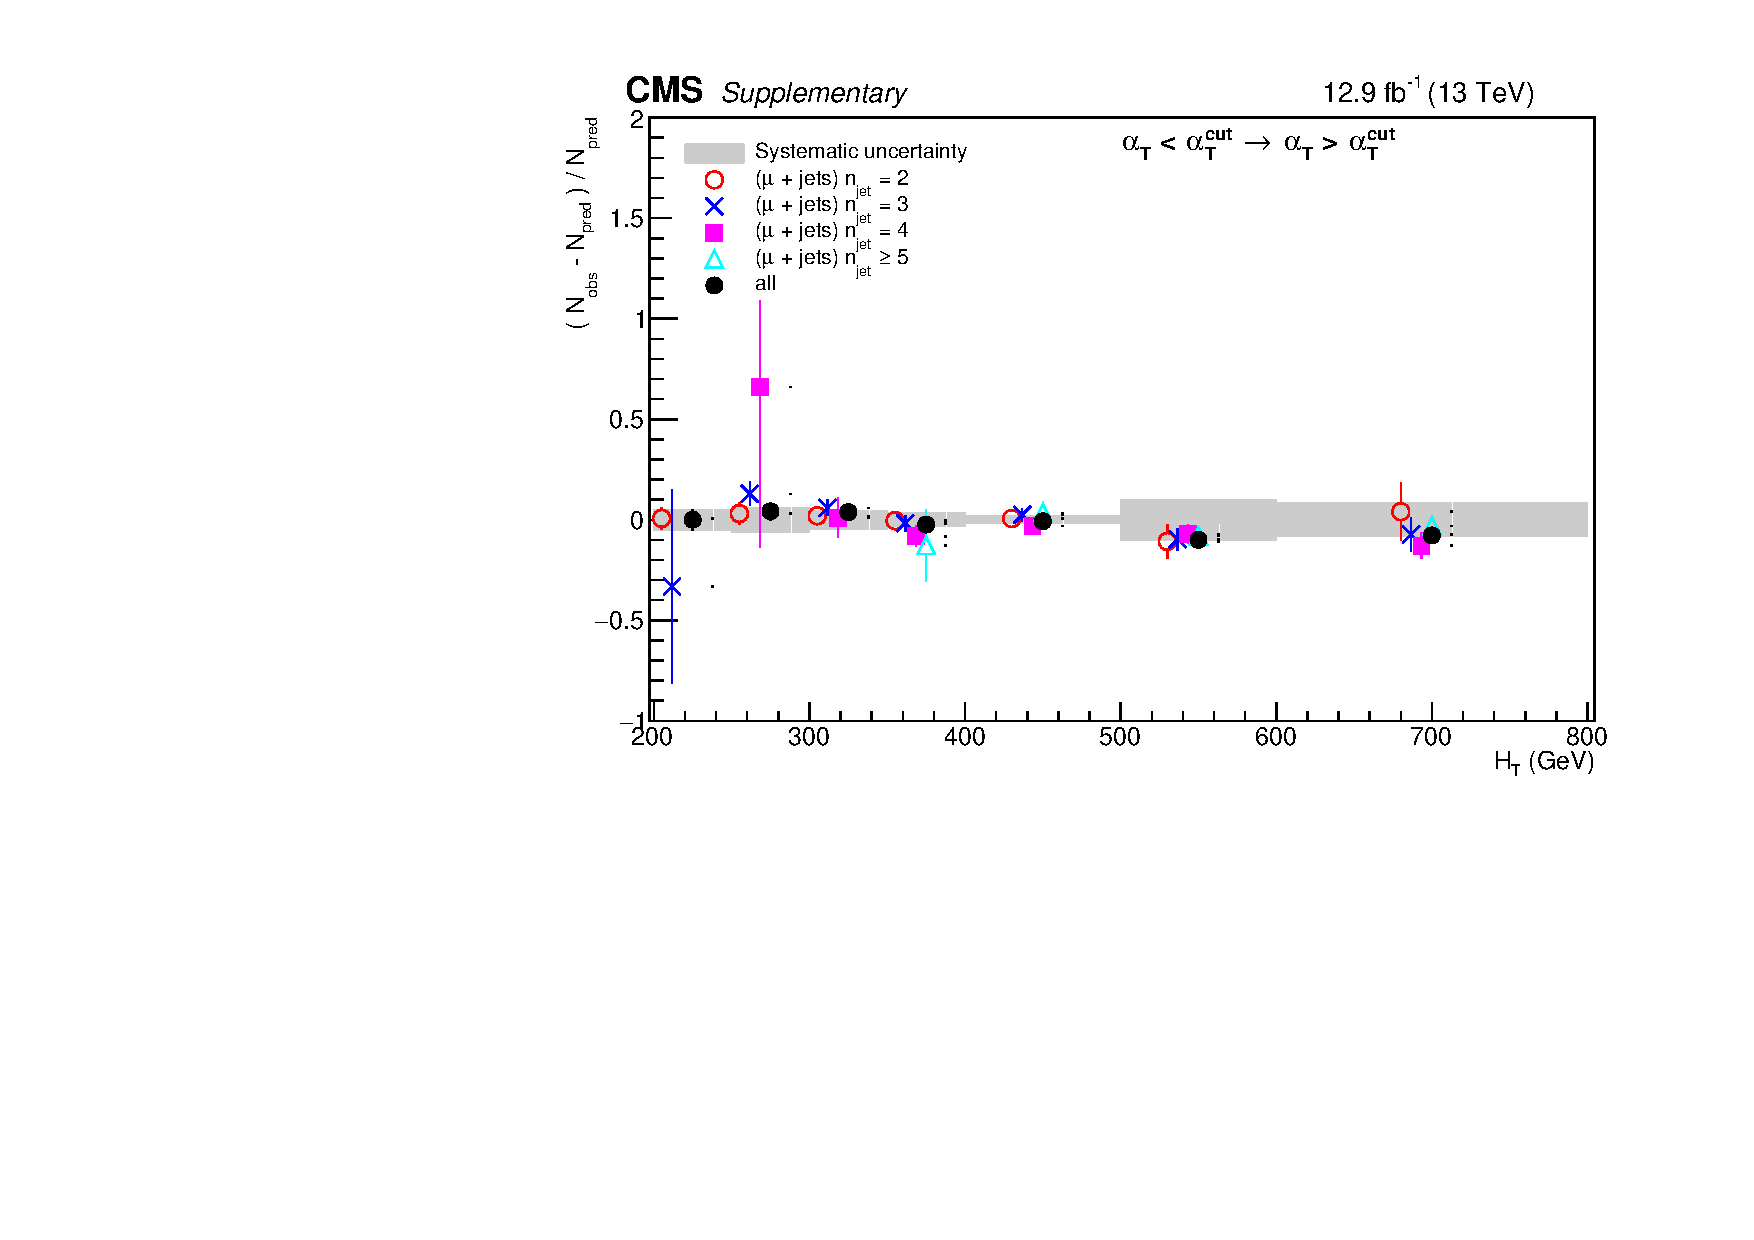
\includegraphics[width=0.5\textwidth]{figs/analysis/closureTests/alphaT_sym__noFit.pdf}}
    ~~
    \subfloat[]{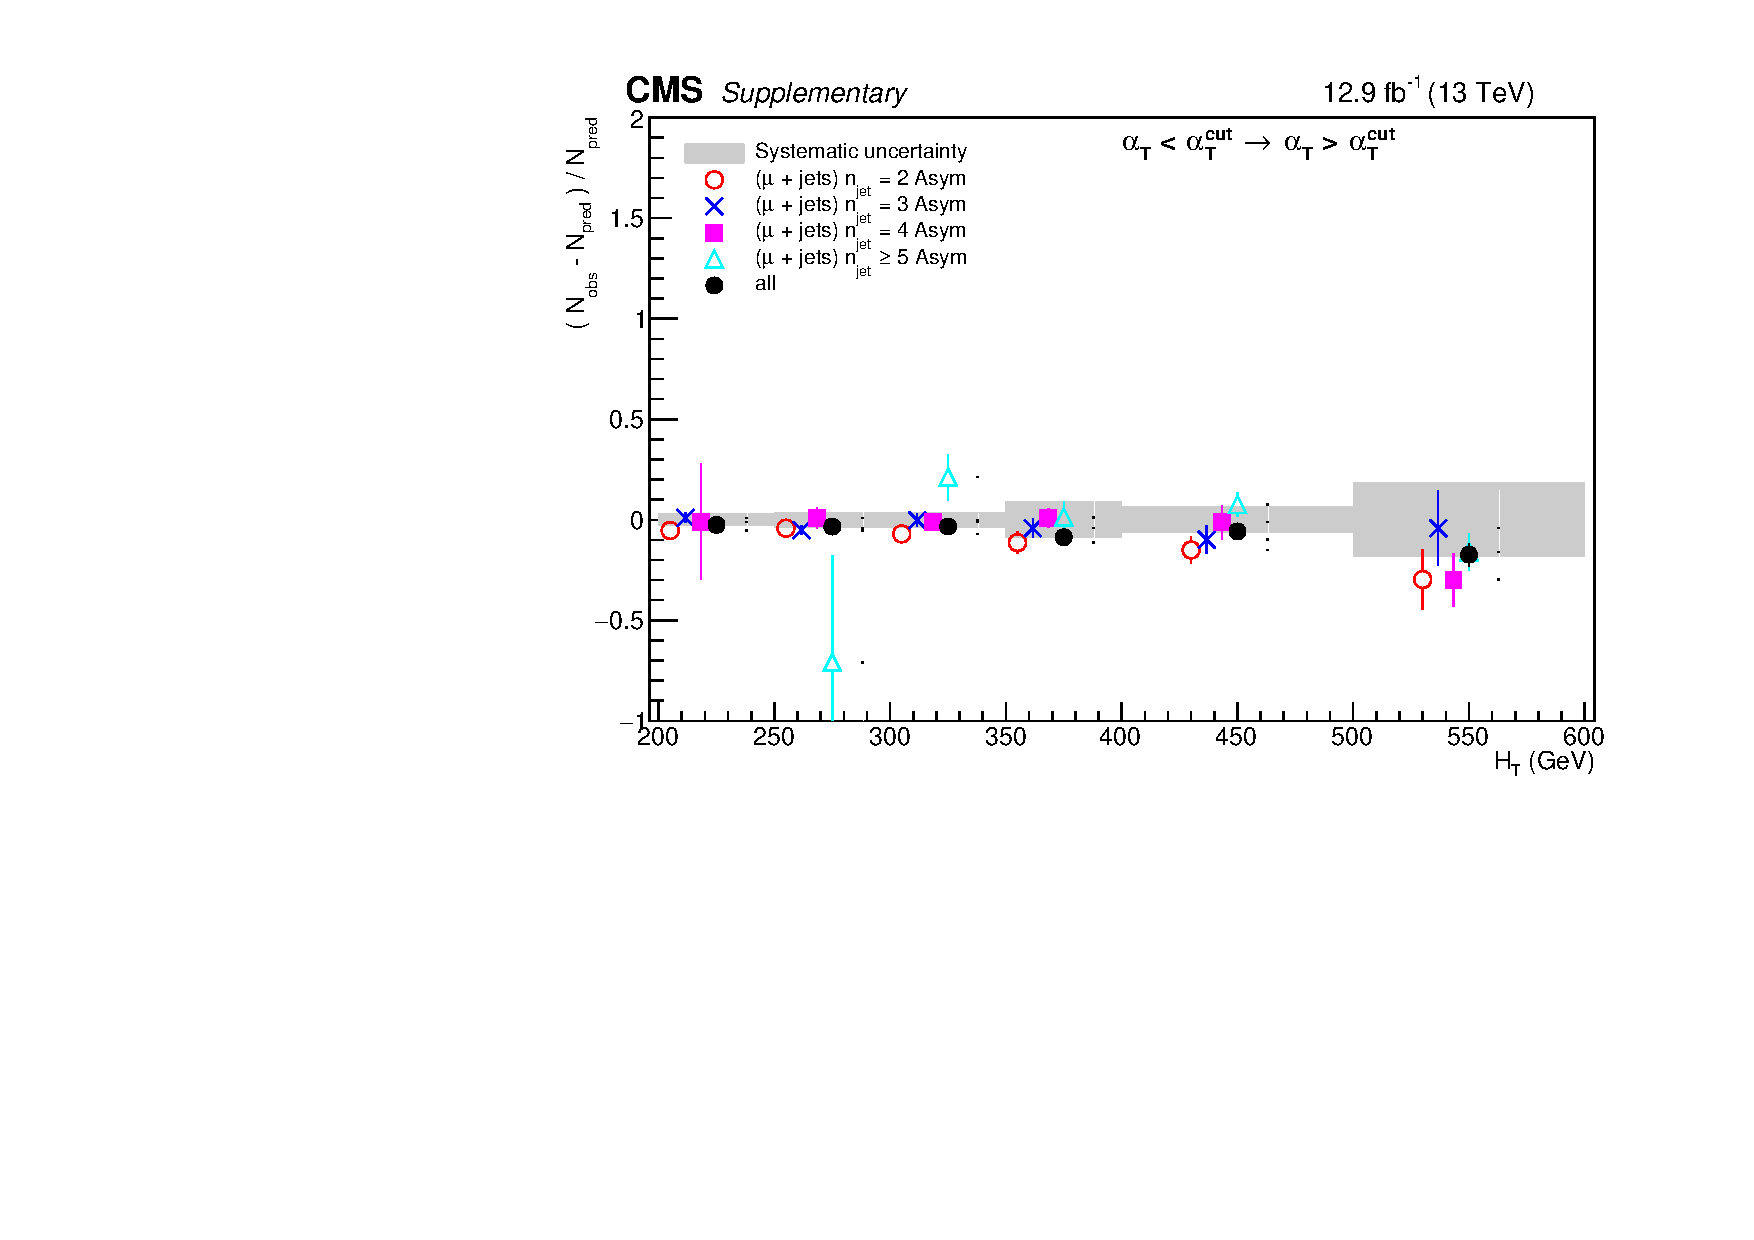
\includegraphics[width=0.5\textwidth]{figs/analysis/closureTests/alphaT_asym__noFit.pdf}}\\
    \subfloat[]{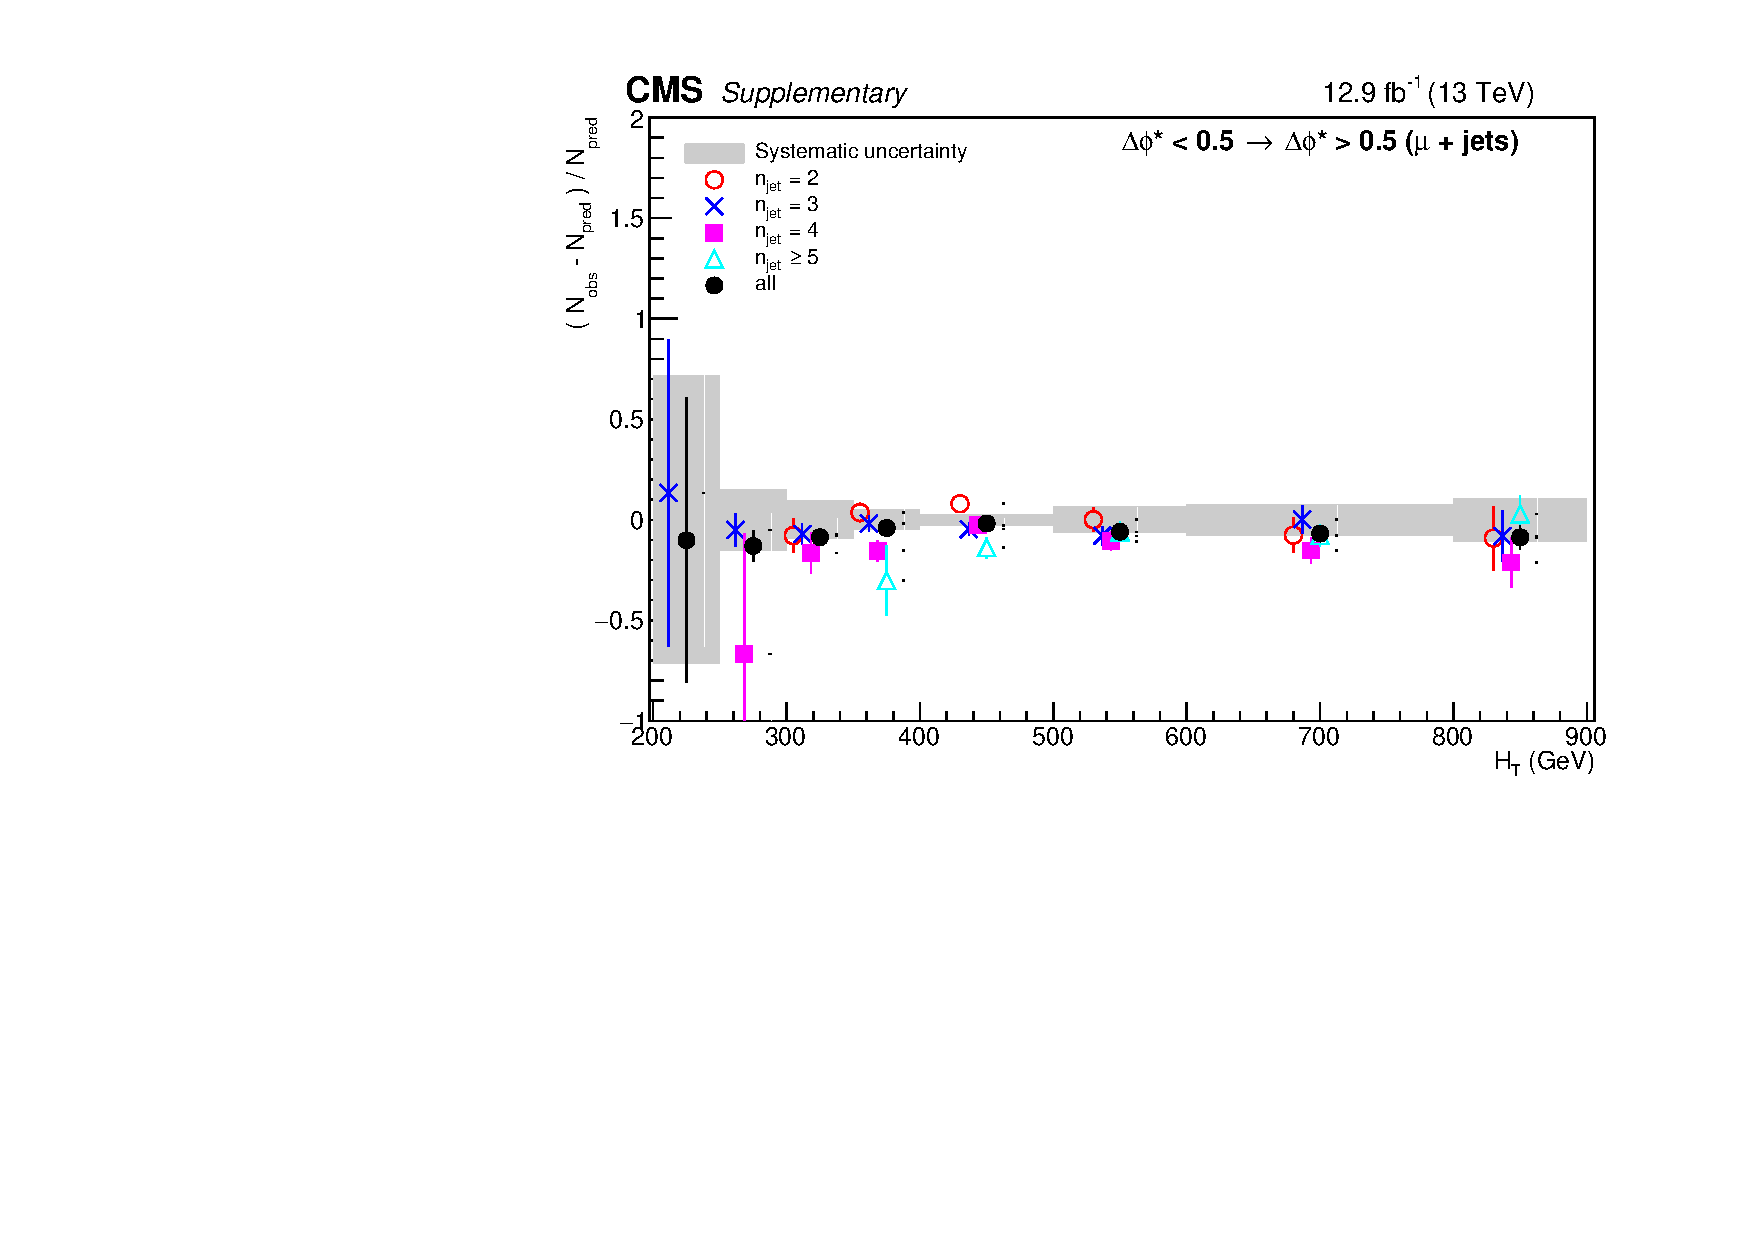
\includegraphics[width=0.5\textwidth]{figs/analysis/closureTests/bDPhi_sym__noFit.pdf}}
    ~~
    \subfloat[]{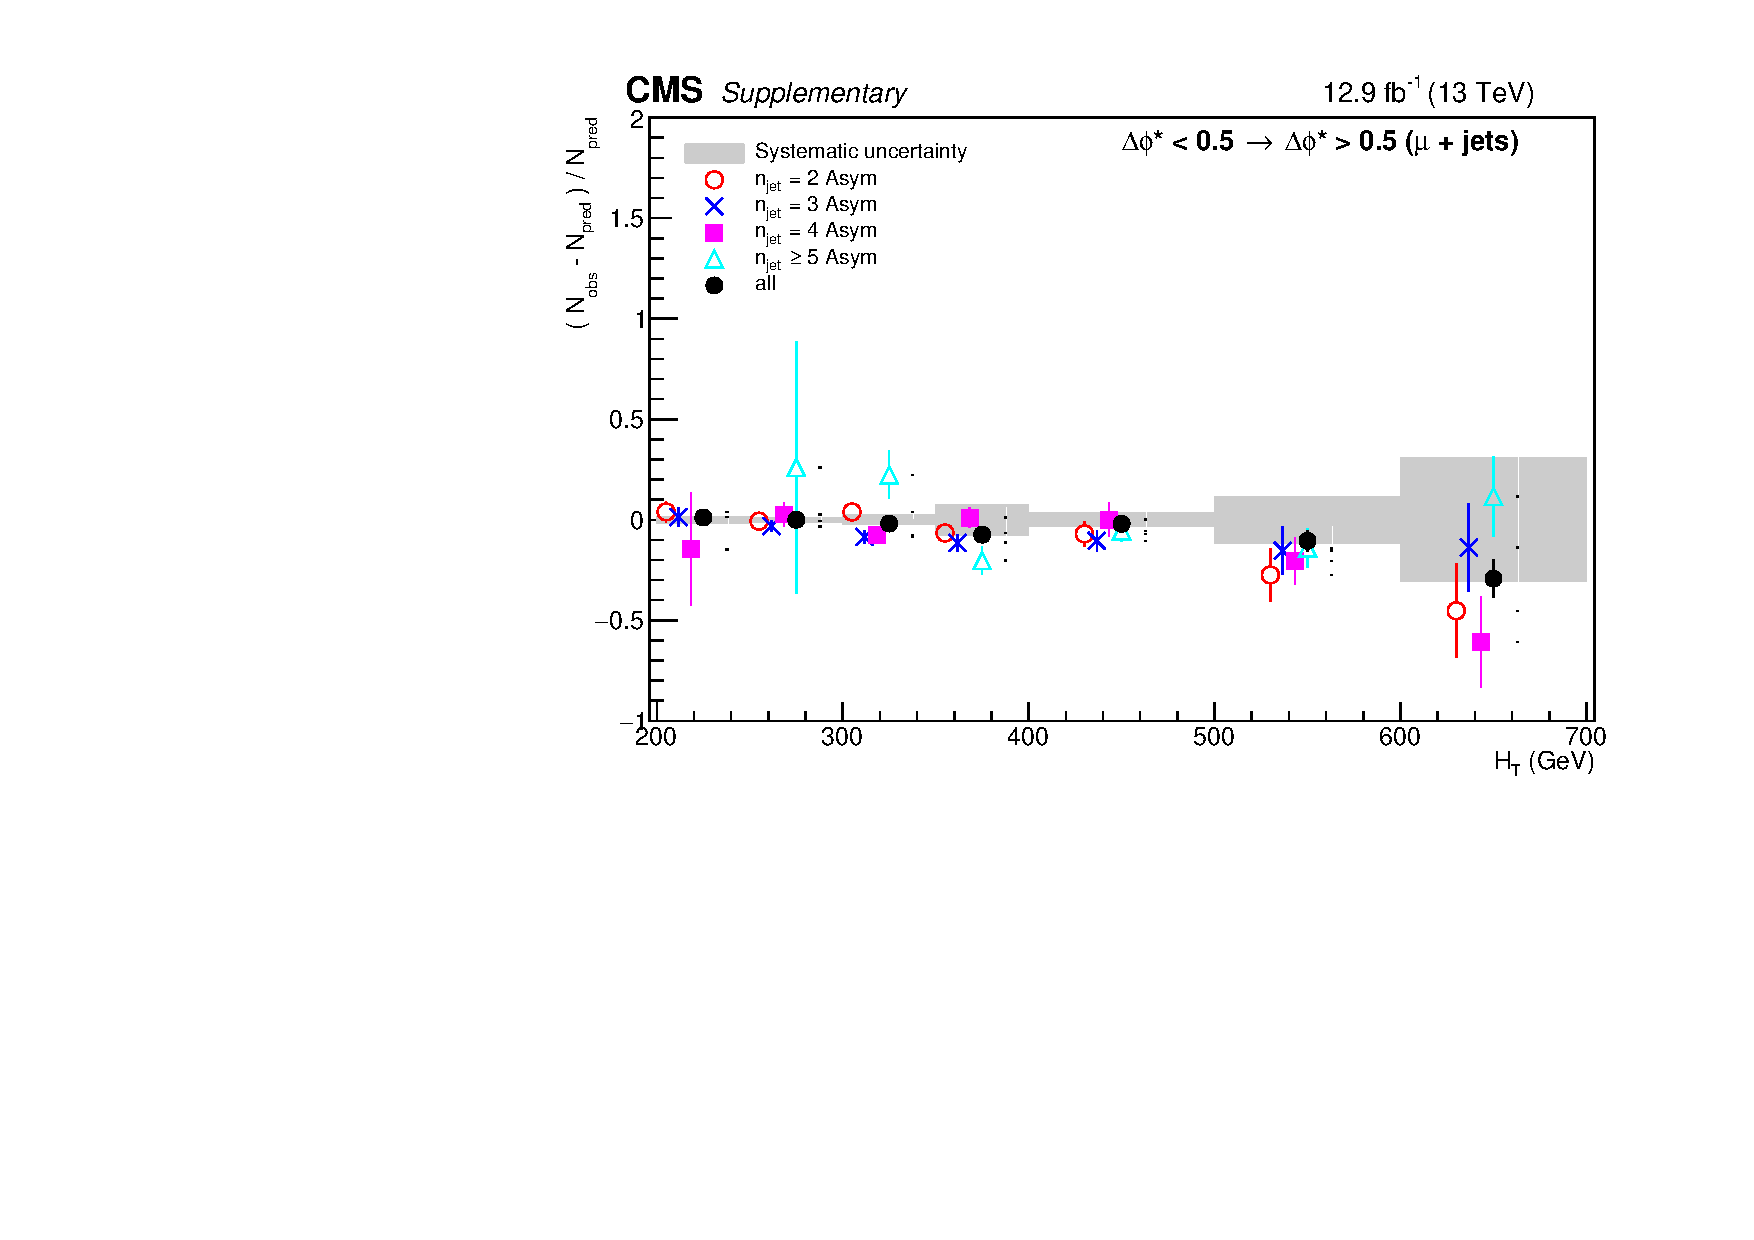
\includegraphics[width=0.5\textwidth]{figs/analysis/closureTests/bDPhi_asym__noFit.pdf}} 

    \caption{Data-driven tests probing the \alphat (top row) and \bdphi (bottom row) extrapolation for each
      \njet category (open symbols) overlaid on top of the systematic
      uncertainty estimates used for each of the seven \scalht bins (shaded bands). 
      The symmetric (asymmetric) jet topologies are shown in the left (right) plot. 
    }
    \label{fig:closureAlphaT}
  \end{center} 
\end{figure}

\subsubsection*{Modelling of the W/Z ratio}
\label{sec:tfSyst_WZratio}
To validate the use of \wmj and \ttbar dominated \mj events to predict
the \znunu background, tests are performed in data using single-muon
and double-muon control regions.  The events in the \mj control region are
used to predict events in the \mmj control region, using transfer
factors from simulation.  These tests target the modelling of the W/Z
ratio in simulation and also indirectly test muon acceptance effects,
which are expected to be sub-dominant and whose uncertainties are
already addressed elsewhere.

The result are shown in Fig.~\ref{fig:closureMuToMuMu} as a function
of \scalht and \njet.  The grey band is the systematic uncertainty
propagated through the analysis, taken as un-correlated per each
\scalht bin and jet topology (symmetric/asymmetric). The systematic
derived from these tests is in the range $3-20\%$.

\begin{figure}[h!]
  \begin{center}
    \subfloat[]{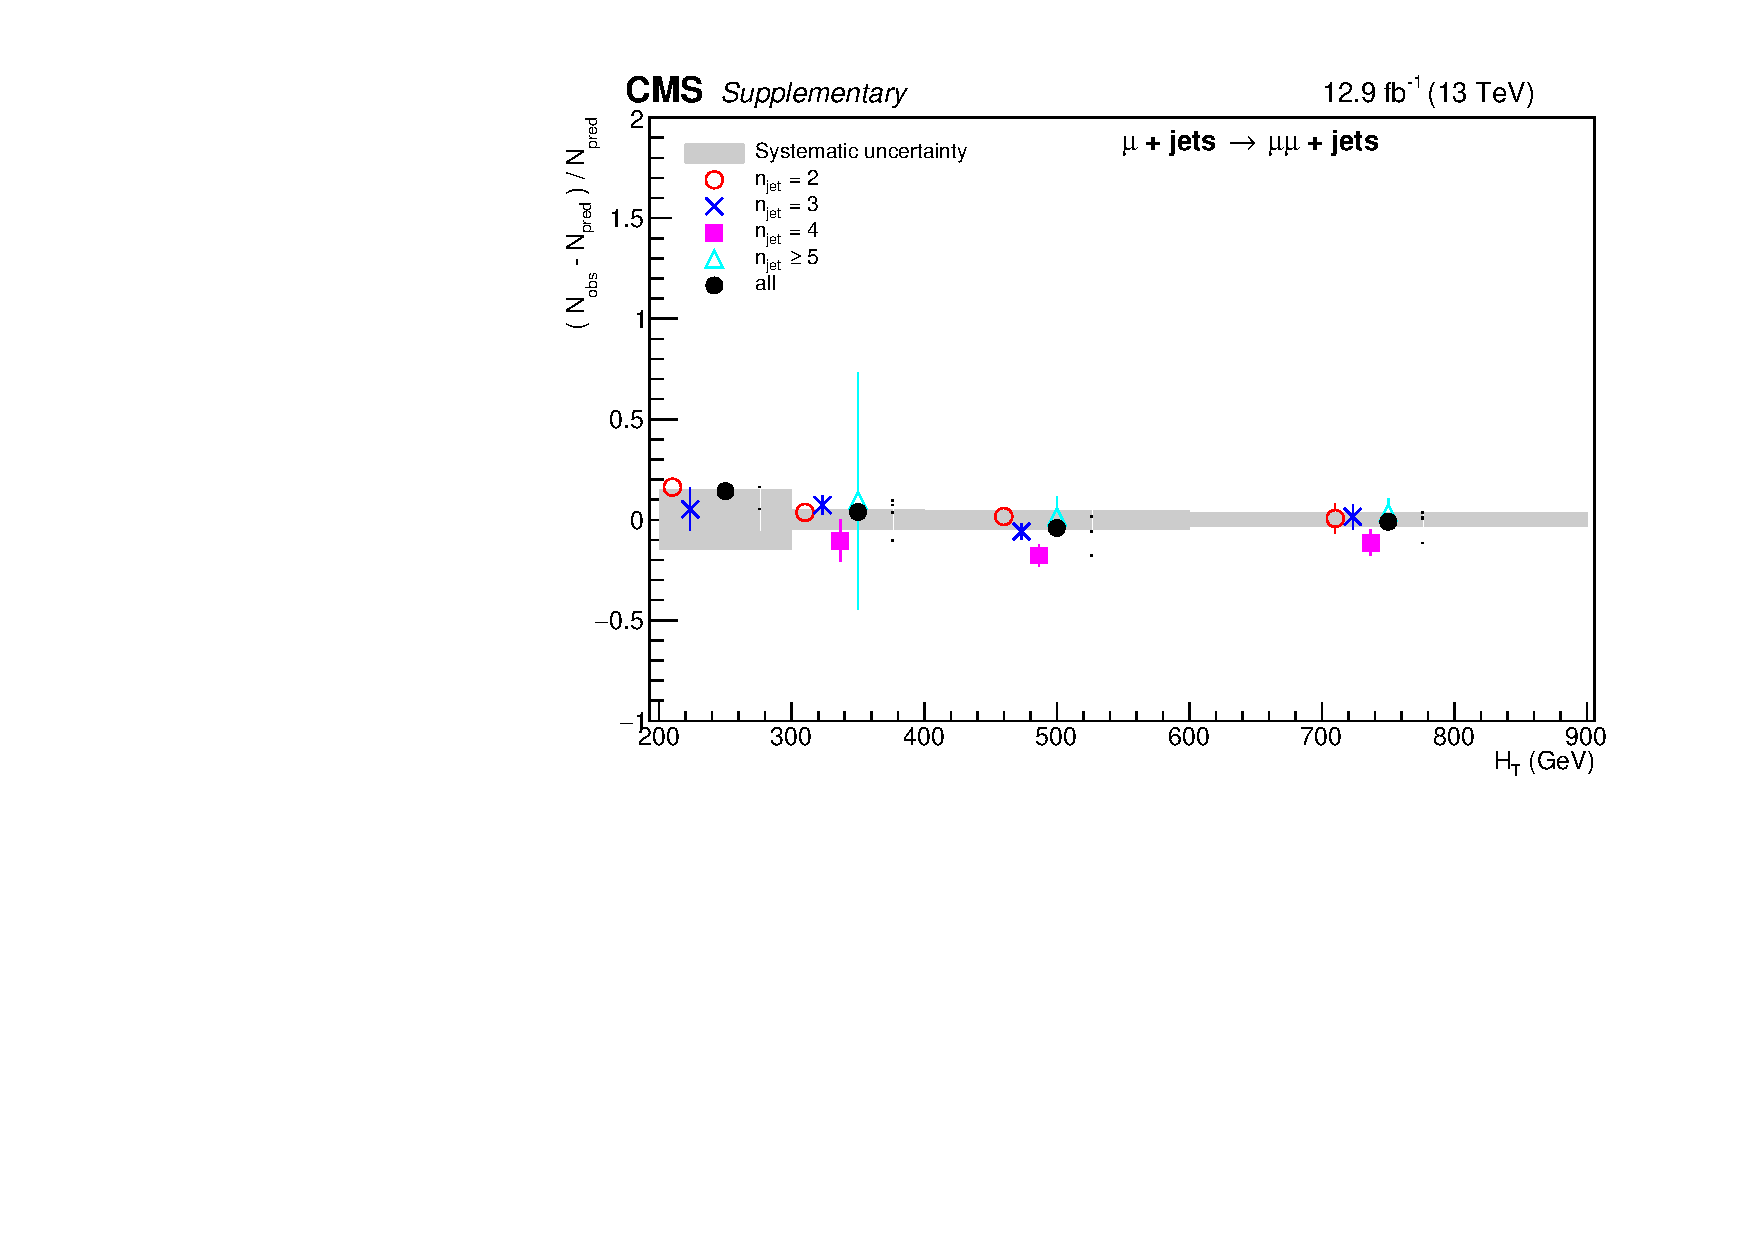
\includegraphics[width=0.5\textwidth]{figs/analysis/closureTests/mu_mumu_sym_half_noFit.pdf}}
    ~~
    \subfloat[]{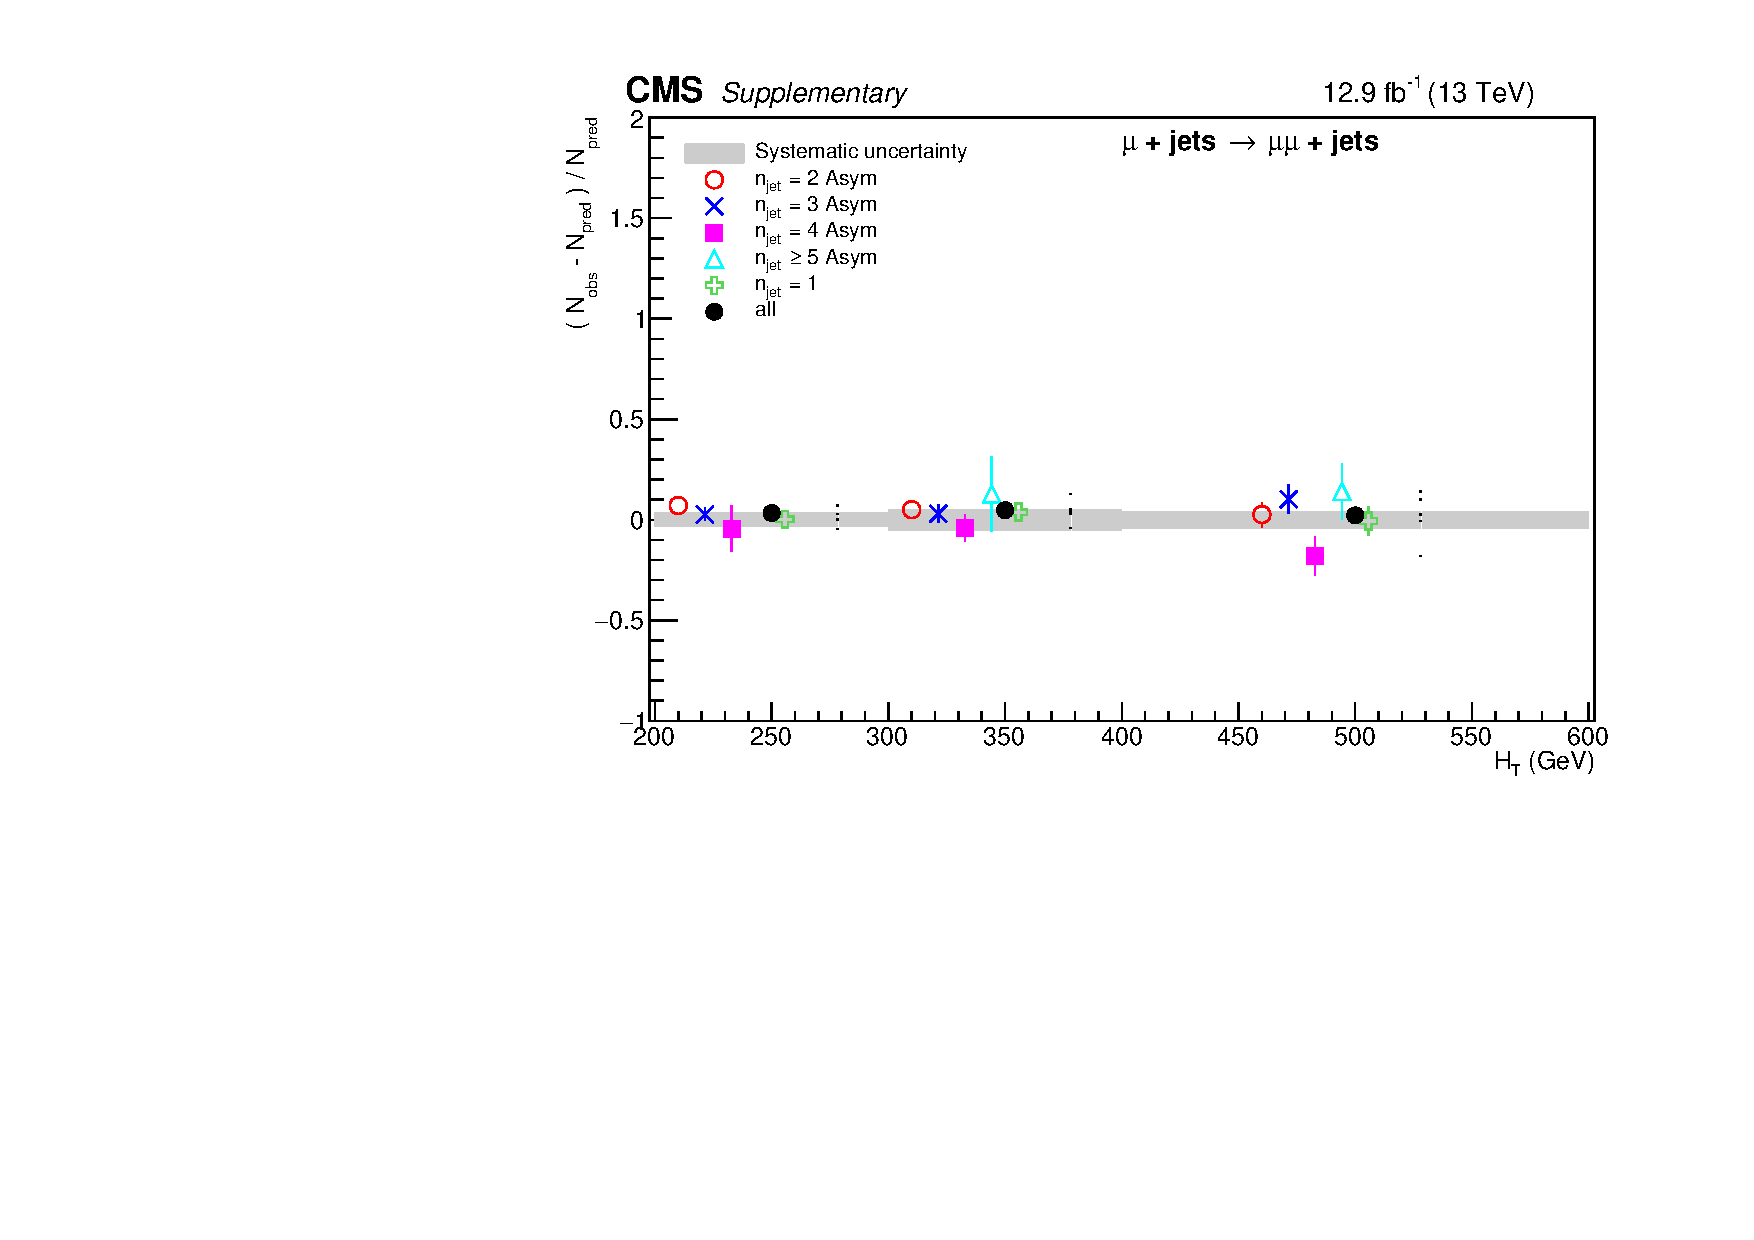
\includegraphics[width=0.5\textwidth]{figs/analysis/closureTests/mu_mumu_asym_half_noFit.pdf}} 
    \caption{Data-driven tests probing the use of the \mj control sample
      to predict the \znunu background for each
      \njet category (open symbols) overlaid on top of the systematic
      uncertainty estimates used for each of the seven \scalht bins (shaded bands).  
      The symmetric (asymmetric) jet topologies are shown in the left (right) plot. 
    }
    \label{fig:closureMuToMuMu}
  \end{center} 
\end{figure}

\subsubsection*{Modelling of the W/Z acceptance due to polarisation effects}
\label{sec:tfSyst_Wpol}

As the kinematics of $W^+$ and $W^-$ decays are subtly different, a
data-driven test is introduced to check the modelling of this W
polarisation in simulation. In this study, carried on using events in
the \mj control region, $\mu^{+}$ events are used to predict $\mu^{-}$
events.  The production mechanism of W bosons from pp collisions means
high $p_T$ $W$ bosons are predominantly left handed \cite{WPol}.  For
high $p_T$ bosons, this implies that $W^+$ decays to the left handed
neutrino along its direction of motion while the lepton is pointing
backward.  The opposite behaviour is expected for the $W^-$. The
lepton is therefore more boosted (and the neutrino less boosted) in
$W^+$ decays than $W^-$ decays.  This leads to a larger number of
$W^+$ decays in the single lepton control regions (which relies on the
lepton $p_T$ for acceptance) than in the signal region (which relies
on the neutrino $p_T$ for acceptance).

The results are shown in Fig.~\ref{fig:closureMuPToMuM} as a function
of \scalht and \njet.  The grey band is the systematic uncertainty
propagated through the analysis, taken as un-correlated per each
\scalht bin and jet topology (symmetric/asymmetric). The systematic
derived from these tests is in the range $3-12\%$.

\begin{figure}[h!]
  \begin{center}
    \subfloat[]{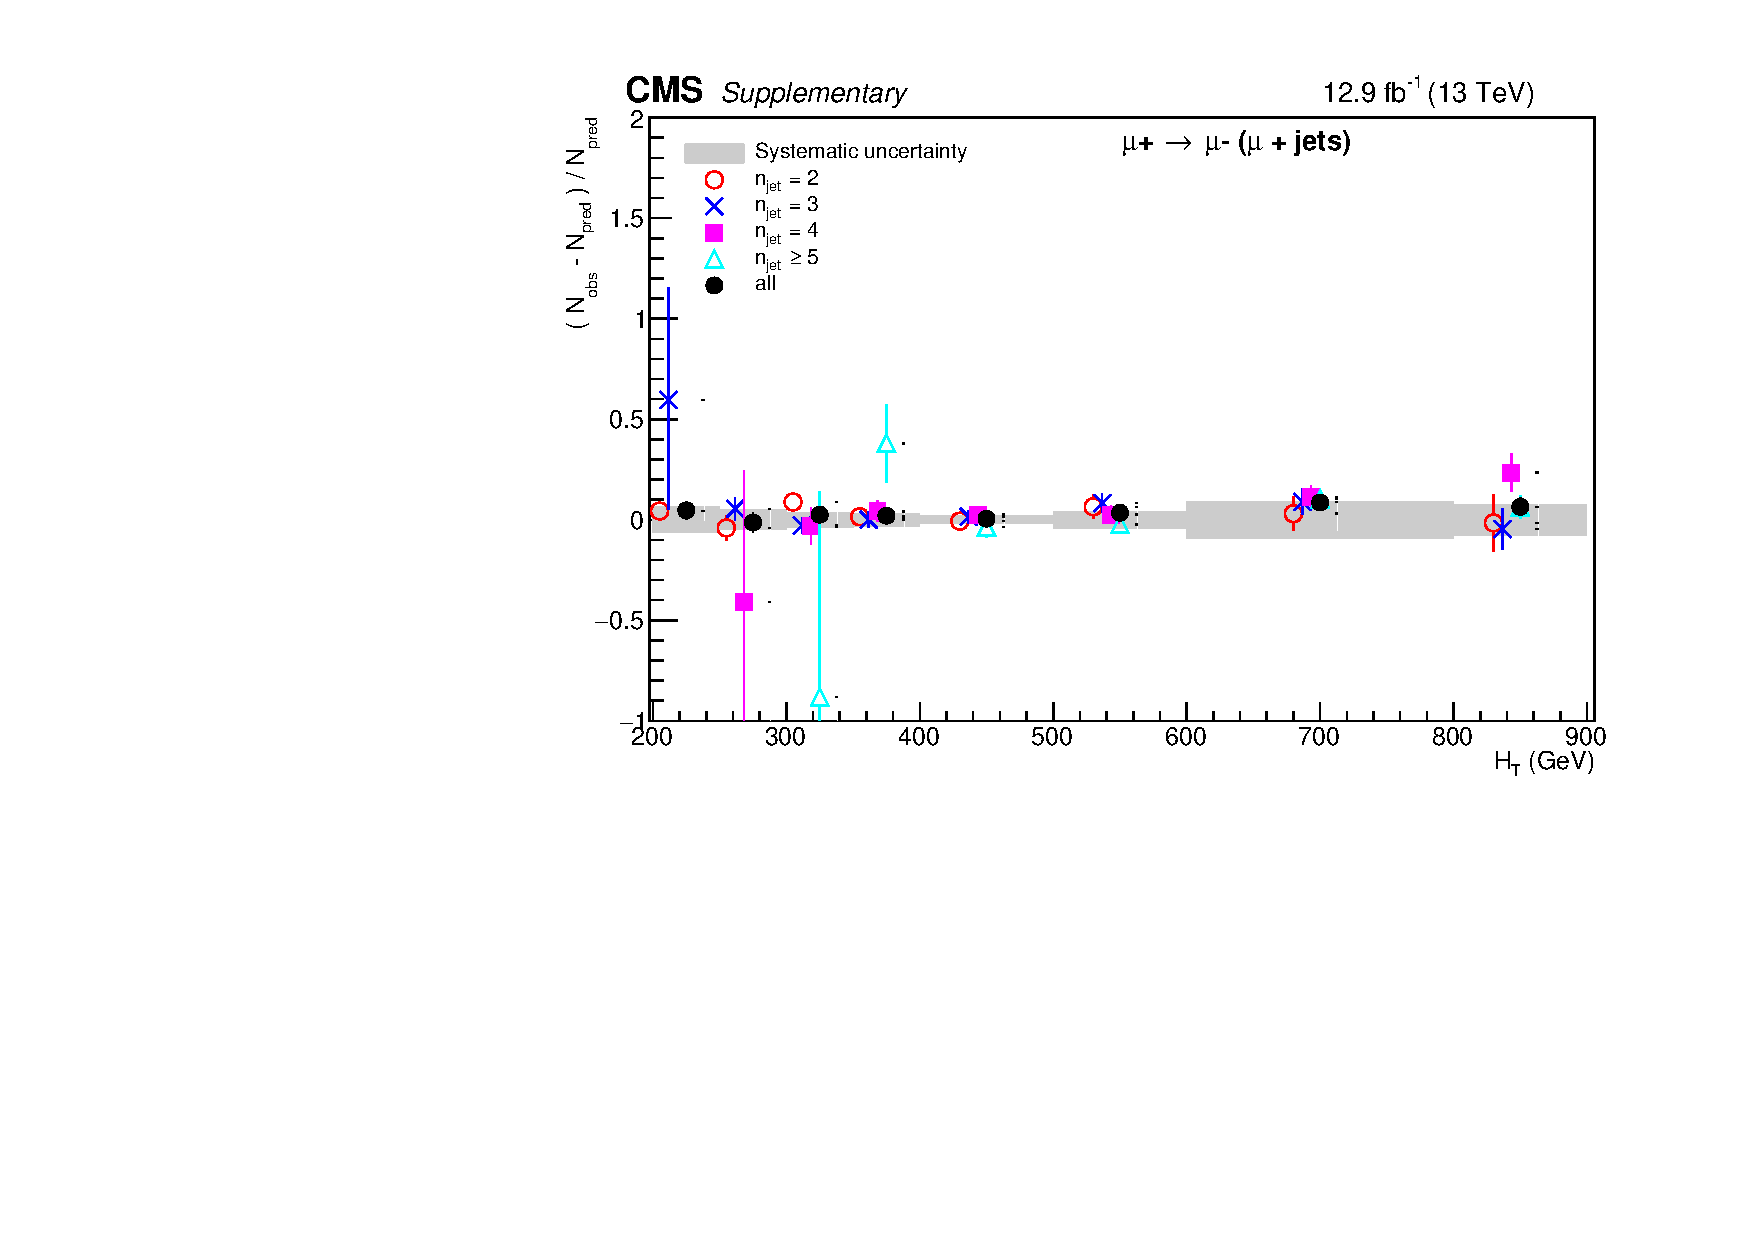
\includegraphics[width=0.5\textwidth]{figs/analysis/closureTests/muplus_muminus_sym__noFit.pdf}}
    ~~
    \subfloat[]{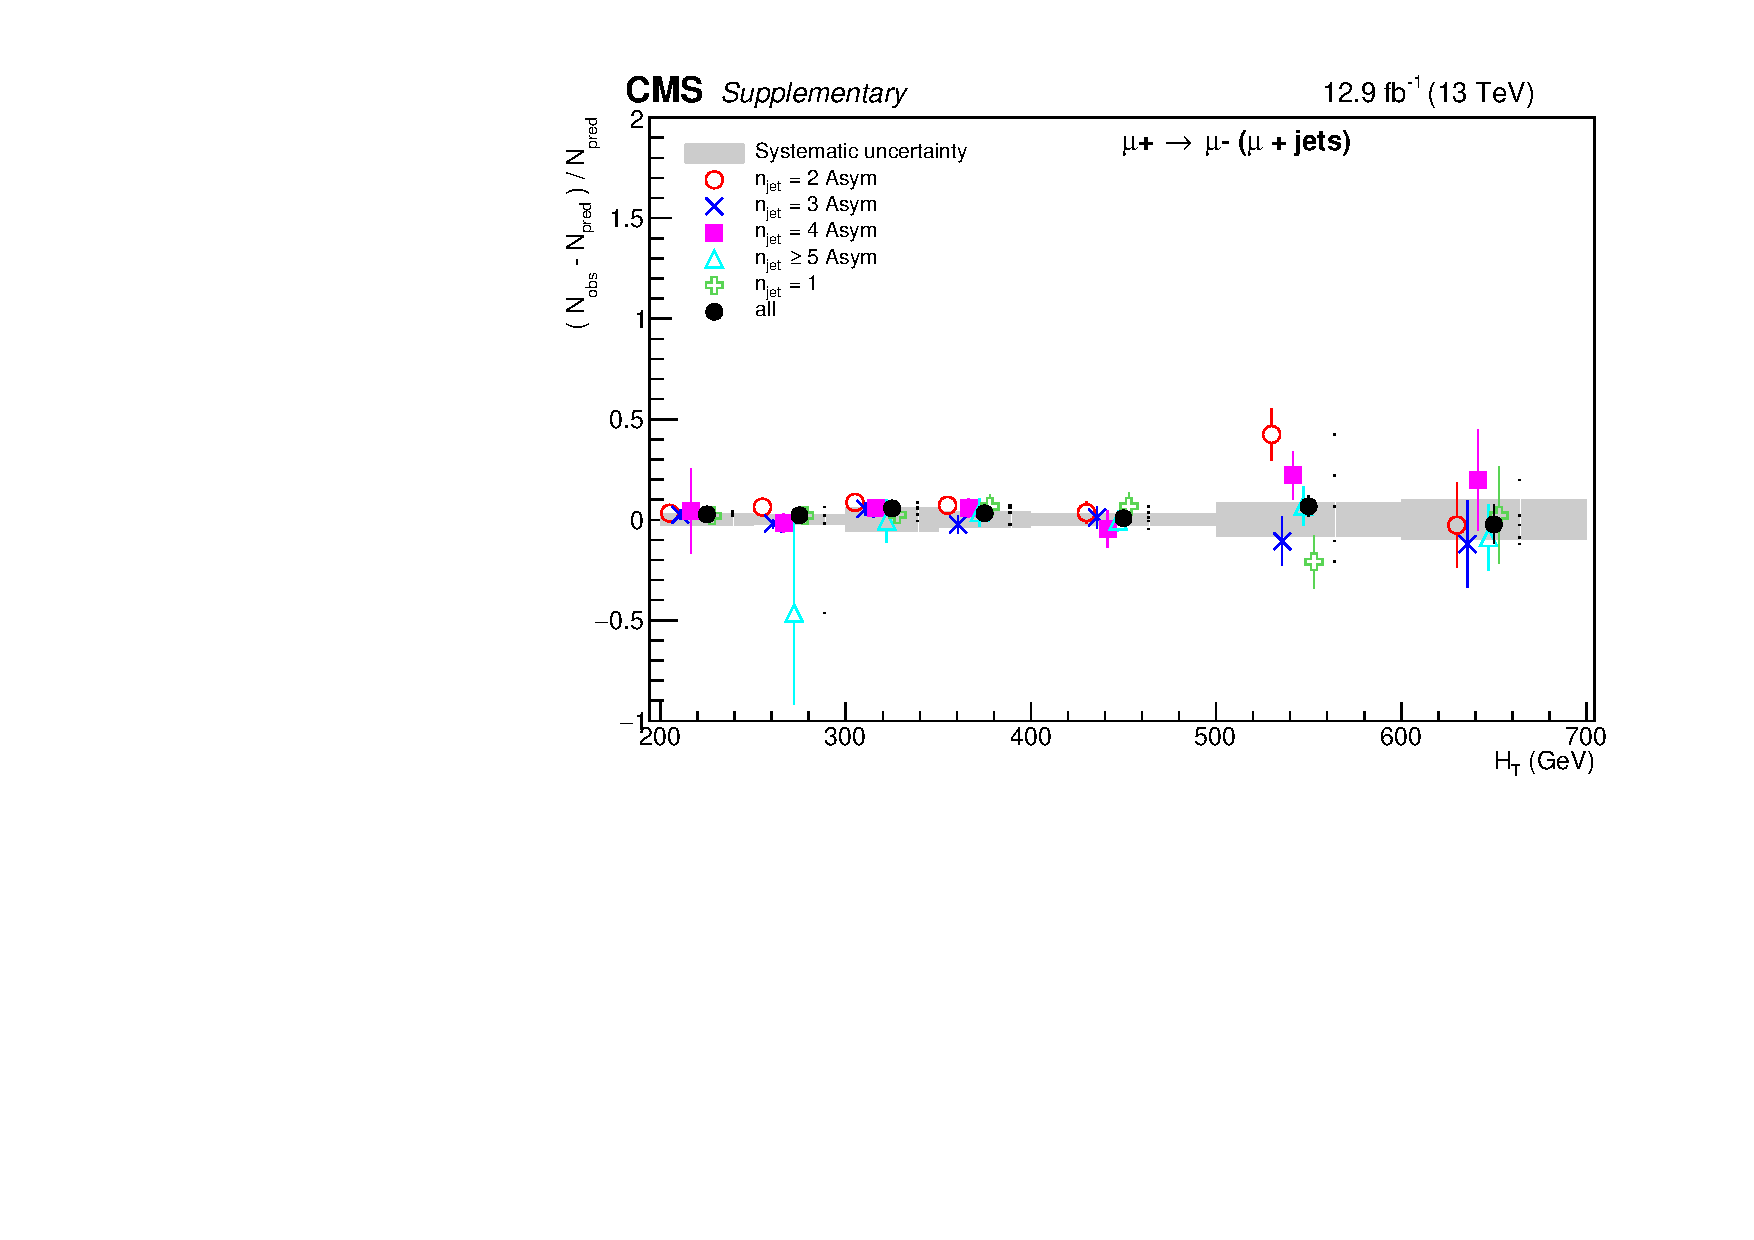
\includegraphics[width=0.5\textwidth]{figs/analysis/closureTests/muplus_muminus_asym__noFit.pdf}} 
    \caption{Data-driven tests probing the W polarisation effects. 
      These are shown for each
      \njet category (open symbols) overlaid on top of the systematic
      uncertainty estimates used for each of the seven \scalht bins
      (shaded bands). 
      The symmetric (asymmetric) jet topologies are shown in the left (right) plot.       
    }
    \label{fig:closureMuPToMuM}
  \end{center} 
\end{figure}

\subsubsection*{Modelling of the Z/$\gamma$ ratio}
\label{sec:tfSyst_ZGratio}
To validate the use of \gj events to predict the \znunu background,
tests are performed in data using the photon and double-muon control
regions. The events in the \gj control are used to predict events in
the \mmj control regions, again using transfer factors from simulation.
These tests target the modelling of the Z/$\gamma$ ratio in simulation
and also indirectly test muon/photon acceptance effects, which,
however, are expected to be sub-dominant and whose uncertainties are
already addressed elsewhere. 

The result are shown in Fig.~\ref{fig:closurePhoToMuMu} as a function
of \scalht and \njet.  The grey band is the systematic uncertainty
propagated through the analysis, taken as un-correlated per each
\scalht bin and jet topology (symmetric/asymmetric). The systematic
derived from these tests is in the range $7-15\%$.

\begin{figure}[h!]
  \begin{center}
    \subfloat[]{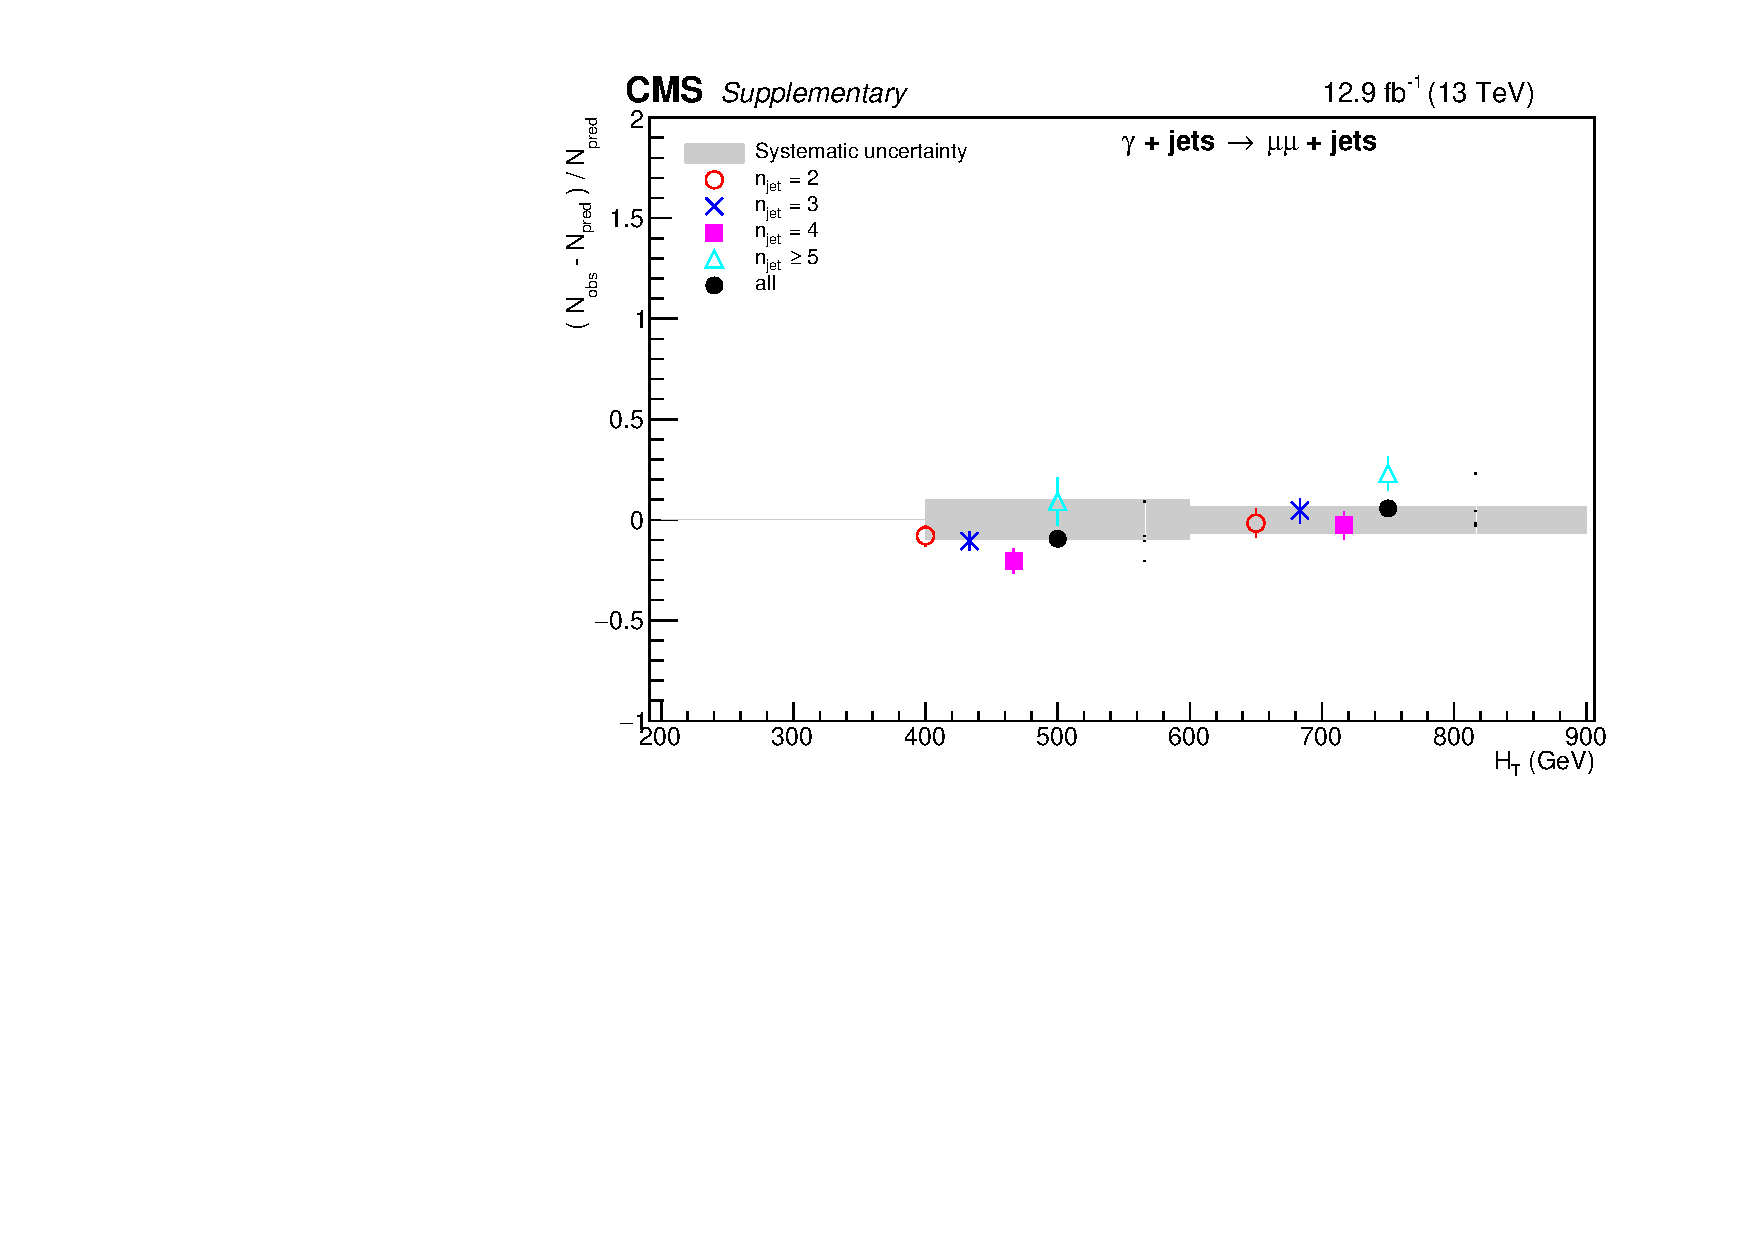
\includegraphics[width=0.5\textwidth]{figs/analysis/closureTests/phot_mumu_sym_half_noFit.pdf}}
    ~~
    \subfloat[]{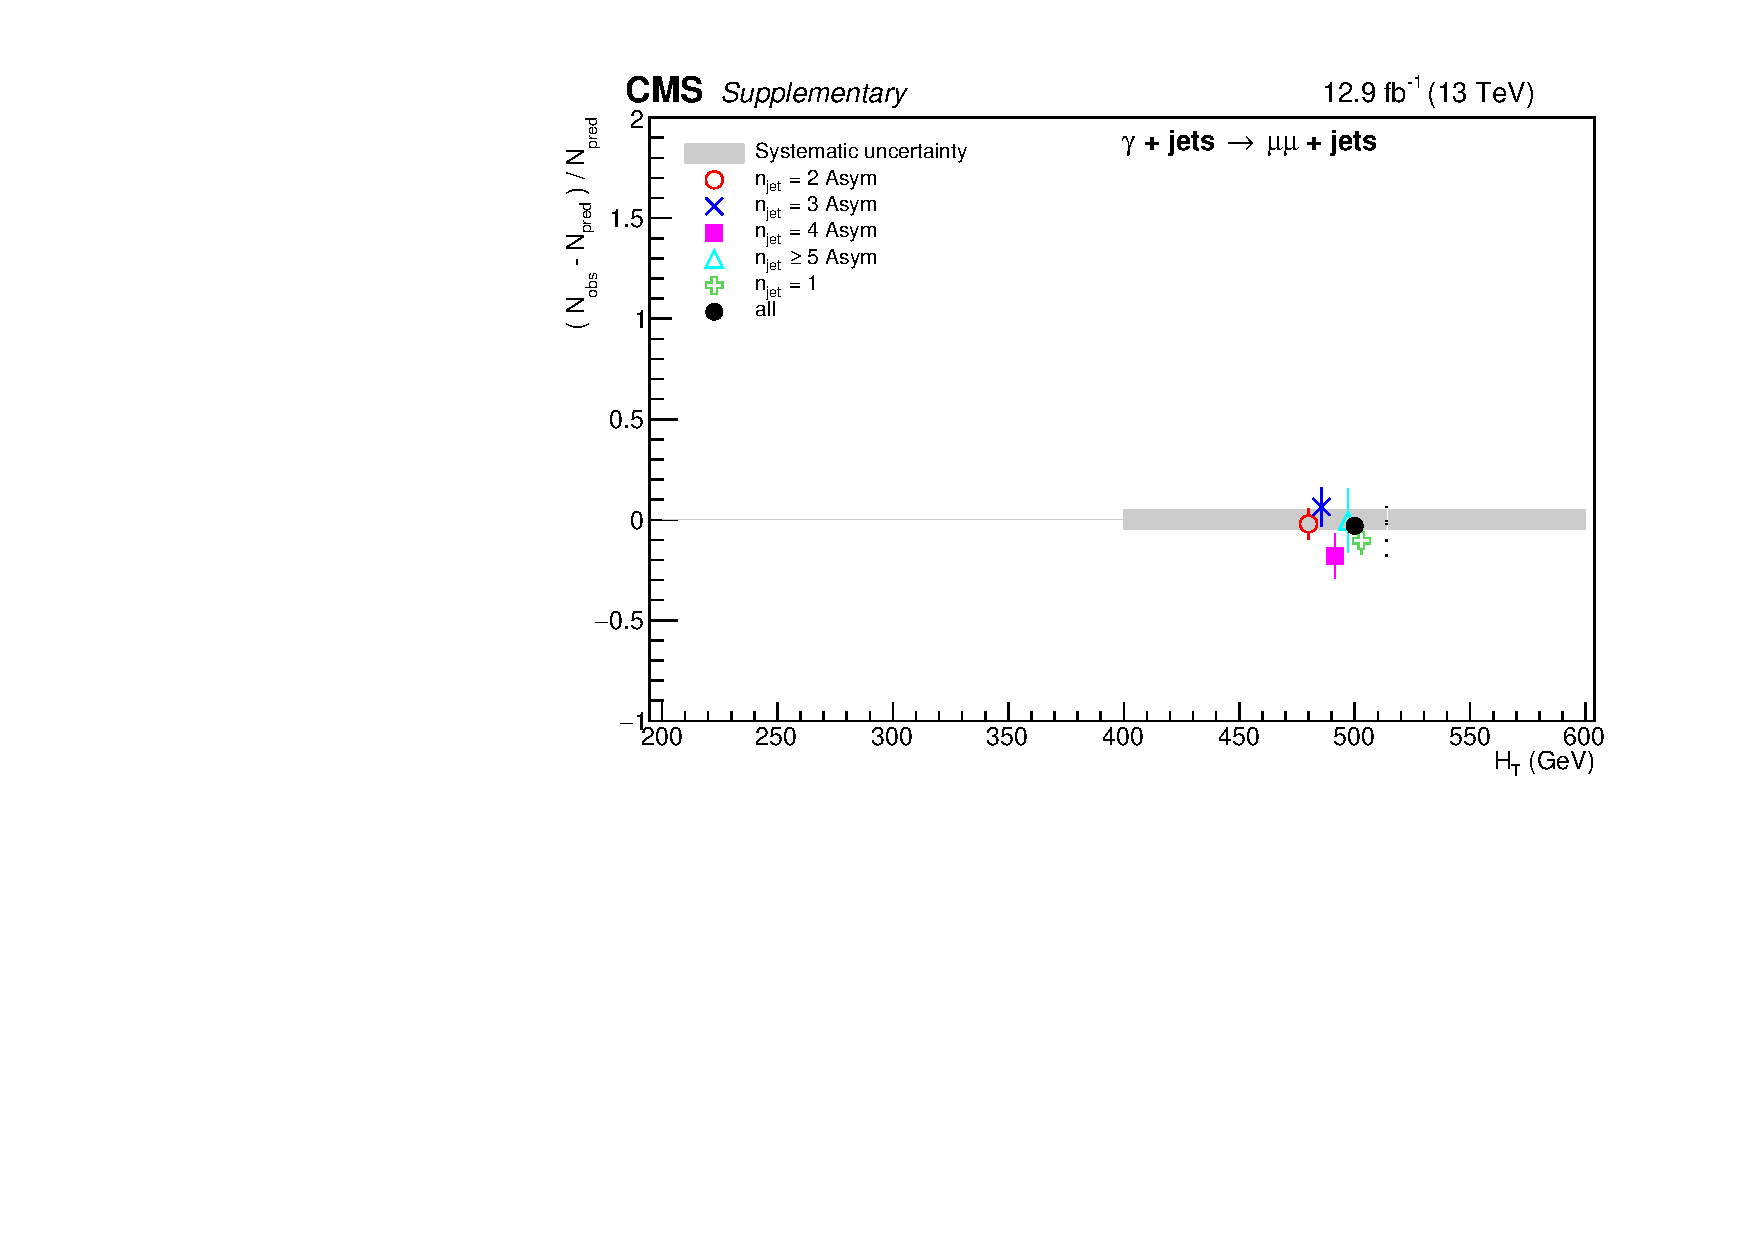
\includegraphics[width=0.5\textwidth]{figs/analysis/closureTests/phot_mumu_asym_half_noFit.pdf}} 
    \caption{Data-driven tests probing the Z/$\gamma$ ratio for each
      \njet category (open symbols) overlaid on top of the systematic
      uncertainty estimates used for each of the seven \scalht bins
      (shaded bands). 
      The symmetric (asymmetric) jet topologies are shown in the left (right) plot.      
    }
    \label{fig:closurePhoToMuMu}
  \end{center} 
\end{figure}

\subsubsection*{Modelling of the W/\ttbar admixture}
\label{sec:tfSyst_WttAd}

The $0$ b-tag $\rightarrow1$ b-tag data-driven tests in the \mj
control region probe the sensitivity of the transfer factors to the
relative admixture of events from the \wj and \ttbar processes,
since they utilise a W-eniched sample to predict a \ttbar-enriched
sample.  These tests indirectly probe also the modelling of the
b-tagging efficiency, although this systematic effect is expected to
be smaller and is already addressed by the dedicated study presented
in Sec.~\ref{sec:tfSyst_btag}.  These tests can slightly overestimate
the uncertainty, as the admixture changes little between the
\mj sample and the signal region, given that no extrapolation between
different b-tag multiplicities is performed in the estimation of the
background. The uncertainty derived is therefore driven by the
limited statistics available in the control sample. 

The result are shown in Fig.~\ref{fig:closureBTag} as a function of
\HT and \njet.  The grey band is the systematic uncertainty
propagated through the analysis, taken as un-correlated per each
\scalht bin and jet topology (symmetric/asymmetric). The systematic
derived from these tests is in the range $4-25\%$.

\begin{figure}[h!]
  \begin{center}
    \subfloat[]{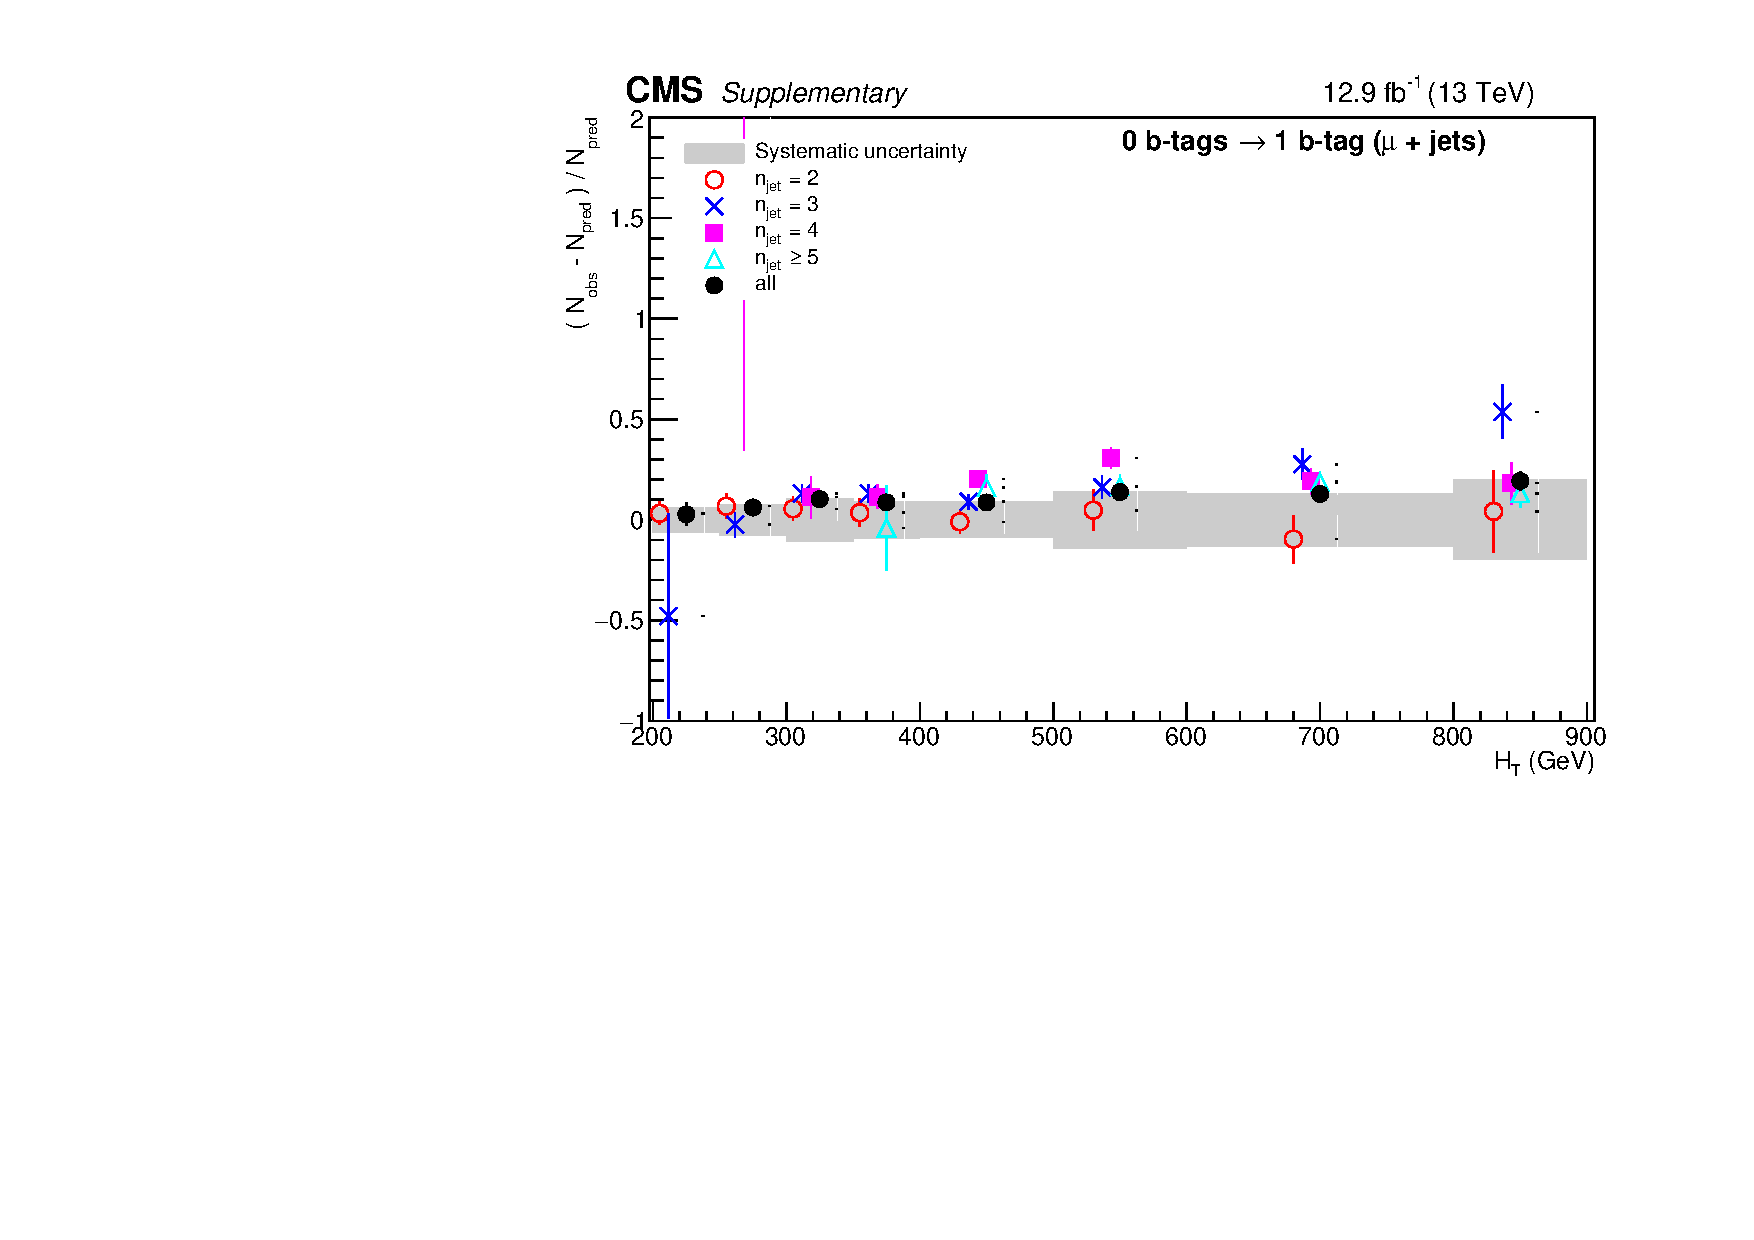
\includegraphics[width=0.5\textwidth]{figs/analysis/closureTests/eq0b_eq1b_muon_sym__noFit.pdf}}
    ~~
    \subfloat[]{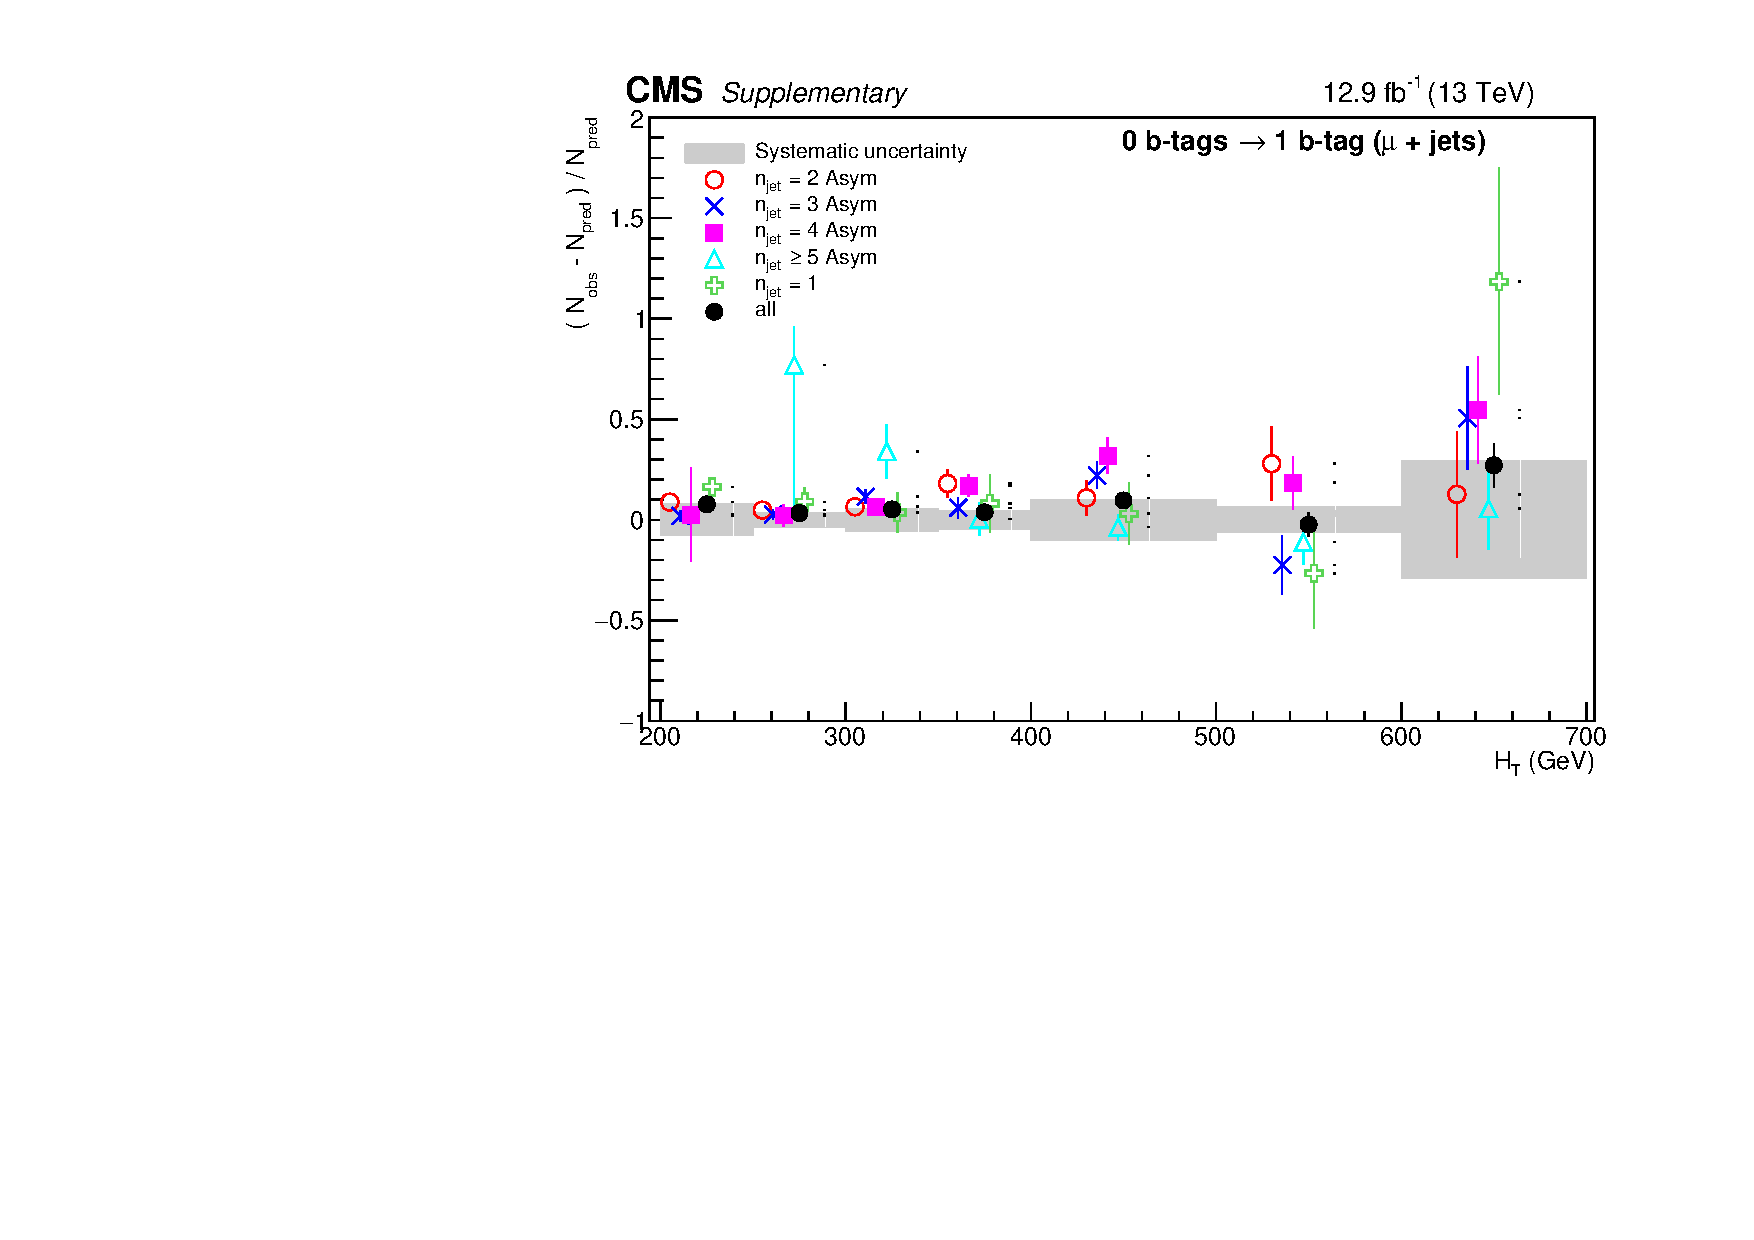
\includegraphics[width=0.5\textwidth]{figs/analysis/closureTests/eq0b_eq1b_muon_asym__noFit.pdf}} 
    \caption{Data-driven tests probing the W and \ttbar admixture 
      in each \njet category (open symbols) overlaid on top of the systematic
      uncertainty estimates used for each of the seven \scalht bins
      (shaded bands). 
      The symmetric (asymmetric) jet topologies are shown in the left (right) plot.      
    }
    \label{fig:closureBTag}
  \end{center} 
\end{figure}

\subsection{Uncertainties in the \MHT dimension}
\label{sec:systMht}

Along with the uncertainty on the \TFs, described above, additional
uncertainties in the shape of the \MHT distribution that is taken from
simulation are derived. For all the known sources of systematic
uncertainty, discussed in Sec.~\ref{sec:simUnc}, the effect of the $\pm 1\sigma$
variation is propagated as uncertainty that varies the \MHT shape.
Due to the fact that the analysis is binned in \HT and \nj bin
migration effects are minimised and these sources of uncertainty are
found to be subdominant.

There is also an uncertainty associated with the fact that the \MHT shape
is taken directly from simulation. To estimate this, a data-driven
method is devised, based on the validation of the \MHT shapes
described in Sec.~\ref{sec:mhtDim}. Within the \mj, \mmj and \gj
control regions the data-simulation ratio of the \MHT shape is
constructed for each (\HT,\nj,\nb) bin. The agreement between the two
distributions is parameterised with a linear orthogonal polynomial.
This function is chosen as it allows one to make a linear fit with
just one parameter as the total overall normalisation is preserved.
To derive the uncertainty for each of the background sources
a simultaneous fit of the \MHT shapes is performed across
all the relevant control regions. This gives a value for the fit
parameter, $p$, which should be compatible with flat, i.e.
$p\approx0$. The uncertainty is then taken as the quadrature sum of
the value of $p$ with its one sigma deviation. This allows alternative
\MHT shapes to be derived based on the $\pm 1\sigma$ variation of this
uncertainty. These alternative shapes are used to encode the
data-driven uncertainty when it is propagated to the final result.

FIXME put in plots comparing to other uncertainties

\newpage
\begin{landscape}
\begin{table}[h!]
  \caption{Summary of the systematics on the transfer factors considered in the analysis, 
    with representatives ranges of uncertainties and the correlation assummed, 
    for the predictions of the $\ttbar$, W and $\znunu$  background
    components.}
  \label{tab:systs}
  \centering
  \footnotesize
  \begin{tabular}{ ccccccc }
    \hline
    \hline
    Systematic & Method & \multicolumn{4}{c}{Relative uncertainty on transfer factor} & Correlation model \\    
     & & $\mj \rightarrow$  & $\mmj \rightarrow$ & $\gj \rightarrow$ & $\mj \rightarrow$ & \\
     & & $\znunu$  & $\znunu$ & $\znunu$ & $\ttbar+W$ & \\
    \hline
    \alphat/\bdphi extrapolation & data-driven tests & $3-30\%$ & $3-30\%$ & - & $3-30\%$ & un-correlated across \scalht/jet top. \\
    W/Z ratio & data-driven tests & $4-15\%$ & - & - & - & un-correlated across \scalht/jet top. \\
    Z/$\gamma$ ratio & data-driven tests & - & - & $6-11\%$ & - & un-correlated across \scalht/jet top. \\
    W/\ttbar admixture & data-driven tests & - & - & - & $4-30\%$ & un-correlated across \scalht/jet top. \\
    W polarisation & data-driven tests & $2-10\%$ & - & - & $2-10\%$ & un-correlated across \scalht/jet top. \\
    Jet energy scale & MC variations & $1-5\%$ & $1-5\%$ & $1-5\%$ & $1-5\%$ & fully correlated \\
    B-tagging efficiency b and c jets & MC variations & $1-3\%$ & $1-3\%$ & $1-3\%$ & $1-3\%$ & fully correlated \\
    B-tagging efficiency light jets & MC variations & $1-3\%$ & $1-3\%$ & $1-3\%$ & $1-3\%$ & fully correlated \\
    Pileup weights & MC variations & $0-2\%$ & $0-2\%$ & $0-2\%$ & $0-2\%$ & fully correlated \\
    Top $p_{T}$ weights & MC variations & $1-30\%$  & $1-10\%$ & - & $1-10\%$ & fully correlated \\
    Lepton scale factor & MC variations & $1-3\%$ & $1-3\%$ & - & $1-3\%$ & fully correlated \\
    Signal trigger efficiency & MC variations & $1-2\%$ & $1-2\%$ & $1-2\%$ & $1-2\%$ & fully correlated \\
    Photon trigger efficiency & MC variations & - & - & $1-2\%$ & - & fully correlated \\
    \hline
    \hline
  \end{tabular}
\end{table}

\end{landscape}


%%%%%%%%%%%%%%%%%%%%
\section{The likelihood model}  % day 3
\label{sec:likelihood}

To carry out a full interpretation of the results of the analysis with
appropriate treatment of systematic uncertainties, a likelihood model
is constructed. Events are categorised based on their (\HT,\nj,\nb)
bin, labelled \htcat, in both the signal region and control regions. Additionally, the
signal region is categorised based on the \MHT bins discussed in
Sec.~\ref{sec:mhtDim}. These bins are represented with an additional
index, $i$. Given
that $n^{\htcat}_{\mathrm{had},i}$ is the number of observed events,
$b^{\htcat}_{\mathrm{had},i}$ is the number of predicted background
events and $s^{\htcat}_{\mathrm{had},i}$ is the expected number of
signal events, the likelihood function in each \htcat category is
defined as the product of poisson distributions for each \MHT bin:
% had likelihood
\begin{equation}
\mathcal{L}^{\htcat}_{\mathrm{had}}=\prod_i
\mathrm{Poisson}(n^{\htcat}_{\mathrm{had},i} |\,
b^{\htcat}_{\mathrm{had},i} + s^{\htcat}_{\mathrm{had},i}).
\label{eq:hadronicLikelihood}
\end{equation}

For each control region, indexed $j$, an independent likelihood
function can be constructed, given $n^{\htcat}_{\mathrm{CR},j}$ is
the number of observed events, $b^{\htcat}_{\mathrm{CR},j}$ is the
number of predicted background events and
$s^{\htcat}_{\mathrm{had},j}$ is the expected signal contamination in
the control region:
% CR likelihood
\begin{equation}
\mathcal{L}^{\htcat}_{\mathrm{CR,j}}=\mathrm{Pois}(n^{\htcat}_{\mathrm{CR,j}}
|\, b^{\htcat}_{\mathrm{CR,j}} + s^{\htcat}_{\mathrm{CR,j}}).
\label{eq:controlLikelihood}
\end{equation}
Due to the way the control regions are selected, the expected signal
contamination is usually found to be negligible.

This results in a total likelihood that is the product over all the
\htcat bins and all the control regions. It can be defined as:
% combined likelihood
\begin{equation}
\label{eq:total_likelihood}
\mathcal{L} = \prod_{\htcat} (\mathcal{L}_{\text{had}}^{\htcat} \times
\prod_{\text{j}} \mathcal{L}_{\text{CR,j}}^{\htcat})
\end{equation}

\subsection{Incorporation of systematic uncertainties}

The background yields in the signal region are connected to the yields
in the control regions through the use of \TFs, as discussed in
Sec.~\ref{sec:TF}. To incorporate this into the fit of the likelihood
model, the yields of the \znunu and combined \ttbar/W backgrounds in
the signal region are correlated with the yields in the control
regions. This is implemented through a single floating parameter
within the fit, which alters the background prediction in the signal
region based on the control region yields and the \TF for each
category. With this implementation, the systematic uncertainties on
each \TF can be properly taken into account when making the background
prediction in the signal region. 

The data-driven uncertainties on the \TFs, described in
Sec.~\ref{sec:closureTests}, are incorporated into the likelihood
model as Gaussian distributed nuisance parameters that act on the
floating parameter. They depend on the background process and the
control region used and are uncorrelated between each of the \htcat
bins.

The uncertainties on the \TFs determined from simulation, described in
Sec.~\ref{sec:simUnc}, are included as \emph{shape} uncertainties on
the \TFs. This means they are fully correlated across all of the
\htcat bins but their magnitude is different depending on the bin. 
Additionally, an uncertainty on the expected signal contribution can
also be taken account as shape uncertainties. These extra
uncertainties depend on the signal model in question and are discussed
in Sec.~\ref{sec:signalModel}.

The uncertainties derived from simulation can also cause bin migration
of events within the \MHT dimension of the signal region. This is
incorporated as a \emph{template} uncertainty, i.e. alternative \MHT
distributions for the $\pm1\sigma$ variation for each of the sources
of uncertainty. 

% (checked this is correct with Matt - depends on the
% analysis, for ICHEP do a simulataneous fit separately for Zinv and
% ttW, uncertainty made from adding p1 in quadrature to p1 unc)
To take account of the uncertainties in the \MHT
distribution, explained in Sec.~\ref{sec:systMht}, additional template
uncertainties are introduced that are decorrelated in \nj and \HT.
Their $\pm1\sigma$ is determined by the uncertainty on the linear fit
used when determining the magnitude of the \MHT uncertainty.
% what about other MHT problem?

Finally, the uncertainty from the limited statistical power of the \MC
samples used is incorporated as an additional nuisance parameter per
\htcat and \MHT bin. This is taken as uncorrelated across all bins.

\subsection{Fitting}

The fit of the likelihood model to find the final result is carried
out in two steps. Firstly, the predicted background yields in the
signal region, $b^{\htcat}_{\mathrm{had}}$, are determined with a fit
in only the control regions, Eq.~\ref{eq:controlLikelihood}. This is
followed by a full fit using the full likelihood model,
Eq.~\ref{eq:total_likelihood}, taking account of all the correlations
between the control regions and signal region, along with the
statistical uncertainties from the
finite number of events in the control region. Within the fit the
likelihood is profiled against all nuisance parameters, which allows
the determination of limits on various signal models. This is
discussed further in Sec.~\ref{sec:signalModel}.

% how the fit is done - split into two components

